\documentclass{article}
\usepackage{commands, caption, subcaption}
\renewcommand{\familydefault}{\sfdefault}
\title{Math 147 Lecture Notes}
\author{Timothy Cho}
\date{December 2023}

\begin{document}
\begin{titlepage}
    \begin{center}
        \vspace*{1cm}
            
        \Huge
        \textbf{UC Irvine Math 147 Fall 2023}
        
        \vspace{0.1 cm}
        \huge
        \textbf{Complex Analysis}
        \vspace{0.4cm}
            
        \vspace{1.5cm}
        \Large    
        \textsf{Professor: Isaac Goldbring}

        \textsf{Teaching Assistant: Michael Hehmann}
        
        \textsf{Notes: Timothy Cho}
            
        \vfill
            

            
        \vspace{0.8cm}
            

        \Large
        December 2023

        Lecture Note Series \#\textbf{2}
            
    \end{center}
\end{titlepage}
\section*{Introduction}
These notes come from both the lecture and the discussion. Sections are numbered chronologically using the following scheme by taking the section number modulo $10$:
\begin{center}
\begin{tabular}{|c|c|c|c|c|}\hline
Date & Lecture & Discussion \\ \hline
Monday & $0$ & $1$  \\
Tuesday & $2$ & $3$ \\
Wednesday & $4$ & $5$ \\
Thursday & $6$ & $7$ \\
Friday & $8$ & $9$ \\ \hline
\end{tabular}
\end{center}
Additionally, the first digit (first two if the section number is three digits long) denotes the week that the lecture/discussion occurred in. It should be noted that not every lecture is recorded in these notes: some lectures were skipped, but despite this the notes should be comprehensible.

The text used was \textit{Complex Variables and Applications}, 9e, by Brown and Churchill. Numbers in [brackets] refer to sections in this text.

\setcounter{section}7
\section{Complex Numbers}
[This is the Week 0 Friday lecture.]

We define the notion of a \textit{complex number}, the objects of study in this course.
\begin{definition}
A \textit{complex number} is an element of the field $\R[x]/\gen{x^2+1}$.
\end{definition}
To an algebraist, this definition makes sense, but it is not very geometric. We can spell this out some more:
\begin{definition}
A \textit{complex number} $z := (a,b)$ is a point in $\R^2$, where addition and multiplication are defined as follows:
$$(a_1, b_1) + (a_2, b_2) := (a_1+a_2, b_1+b_2);$$
$$(a_1, b_1)\cdot (a_2, b_2) := (a_1a_2 - b_1b_2, a_2b_1 + a_1b_2).$$
We will write these points as $z = (a,b) = a + bi$, where we $i := (0, 1)$, and we define the \textit{real} resp. \textit{imaginary} parts of $z$ by $\Re(z) := a$ and $\Im(z) := b$.

The \textit{set} of complex numbers is denoted by $\C$.
\end{definition}
Readers with experience in Math 120B can show the equivalence of these two definitions. Immediately, we get the following consequence, which the reader can verify.
\begin{proposition}
Let $z,w\in\C$. Then $\Re(z+w) = \Re(z) + \Re(w)$ and $\Im(z+w) = \Im(z) + \Im(w)$.
\end{proposition}

Similarly, the reader, using Definition 8.2, can verify the following:
\begin{theorem}
The complex numbers $\C$, as defined in Definition 8.2, form a field.
\end{theorem}

With that being said, division over the complex numbers deserves some special treatment. Take some $z\in \C\setminus\{0\}$. Then since $\C$ is a field, there exists a unique $w\in\C$ such that $zw = 1$. Letting $z = a+bi$, we write
$$w = \frac 1z = \frac1{a+bi} = \frac{a-bi}{a^2+b^2} = \frac a{a^2+b^2} - \frac{b}{a^2+b^2} i,$$
and we leave it for the reader to verify  that
$$zw = (a+bi)\paren{\frac a{a^2+b^2} - \frac b{a^2+b^2}i} =1.$$

We can simplify our formulas from above by introducing two fundamental concepts.
\begin{definition}
Let $z := a+bi$. The \textit{complex conjugate} $\bar z$ is the complex number $\bar z:= a-bi$.
\end{definition}
\begin{definition}
Let $z:=a+bi$. The \textit{modulus} $|z|$ is the real number $|z| := \sqrt{a^2+b^2}$.
\end{definition}
Intuitively, the complex conjugate is the reflection of $z$ about the $x$-axis, and the modulus is the length of $z$ regarded as a vector in $\R^2$. We get the following proposition:
\begin{proposition}
Let $z\in\C$ be nonzero. Then $z^{-1} = \bar z/|z|^2$.
\end{proposition}
Of course, a useful rearrangement of this is as follows:
\begin{corollary}
Let $z\in\C$ be nonzero. Then $z\bar z = |z|^2$.
\end{corollary}
\setcounter{section}9
\section{Complex Conjugation and Polar Form}
\subsection*{[6] Complex Conjugation}
We introduce these basic properties of complex conjugation, which the reader can verify.
\begin{proposition}
Let $z,w\in \C$. Then $\overline{\overline z} = z$, $|\bar z| = |z|$, $\overline{z+w} = \bar z + \bar w$, and $\overline{zw} = \bar z\cdot \bar w$.
\end{proposition}
We can also take the conjugate of the inverse:
\begin{proposition}
Let $z\neq 0$. Then $\overline{z^{-1}} = (\bar z)^{-1}$.
\end{proposition}
\begin{proof}
Recall that $z^{-1} = \bar z/|z|^2$. Then
$$\overline{z^{-1}} = \overline{\paren{\frac{\bar z}{|z|^2}}} = \frac{\overline{\overline z}}{|z|^2} = \frac z{|z|^2},$$
as $|z|^2$ is real, and 
$$(\bar z)^{-1} = \paren{\frac{|\bar z|^2}{\overline{\overline z}}}^{-1} = \frac z{|\bar z|^2} = \frac z{|z|^2} = \overline{z^{-1}}.$$
\end{proof}
Also, we note the following relationships between a complex number and its conjugate:
\begin{proposition}
For any $z\in \C$, we have $\ds \Re(z) = \frac{z+\bar z}2$ and $\Im(z) = \ds\frac{z-\bar z}{2i}$.
\end{proposition}
Finally, the following is true regarding the moduli of complex numbers:
\begin{proposition}
For any $z\in\C$, we have $|zw| = |z||w|$ and $|z^n| = |z|^n$ for any $n\in\N$.
\end{proposition}
\begin{proof}
We have $|zw|^2 = zw\overline{zw} = zw\bar z\bar w = z\bar z\cdot w\bar w = |z|^2|w|^2$, so taking the square root gives us the first of these. Now induct on $n\in\N$.
\end{proof}

We leave it for the reader to show that $|z/w| = |z|/|w|$ when $w$ is nonzero. \newpage
\subsection*{[7] Exponential Form}
Let $z:= x+yi$ be nonzero. We define $r := |z| > 0$, and we define $\theta$ to be the angle between the positive $x$-axis and the vector determined by $z$, measured counterclockwise. By drawing this out and using trigonometry, we establish that
$z = r\cos \theta + ir\sin \theta  = r(\cos \theta + i\sin\theta) =: r\cis \theta$. This allows us to express a complex number in terms of length and angle, but the angle $\theta$ is not unique. We thus define the \textit{argument} of $z := r\cis\theta_0$ to be the set of all $\theta$ such that $r\cis\theta = z$.
\begin{example}
Let $z = 1+i = \sqrt 2\cis(\pi/4)$. Since both sine and cosine are periodic with period $2\pi$, we see that $\cis(\pi/4) = \cis(\pi/4 + 2k\pi)$ for all $k\in\Z$. Hence
$$\arg(1+i) = \boxed{\set{\frac\pi4 + 2k\pi: k\in\Z}},$$
or in algebraic coset notation, $\arg(1+i) = \pi/4 + 2\pi\Z$.
\end{example}
From this infinite set of arguments, we often find it helpful to distinguish the ``preferred" value of the argument.
\begin{definition}
The \textit{principal argument} of $z$, denoted $\Arg z$, is the unique element of $\arg z\cap (-\pi, \pi]$.
\end{definition}
Of course, this uniqueness comes from the fact that sine and cosine have period $2\pi$.

Now, recall from Math 2B that we have the following Taylor series expansion for cosine and sine, and we can write the following:
$$\cos\theta =  \sum_{n=0} ^\infty (-1)^n \frac{\theta^{2n}}{(2n)!} = \sum_{n=0}^\infty i^{2n}\frac{\theta^{2n}}{(2n)!},\textsf{ and}$$
$$i\sin\theta = i\sum_{n=0}^\infty (-1)^n \frac{\theta^{2n+1}}{(2n+1)!} = \sum_{n=0}^\infty \frac{i^{2n+1}\theta^{2n+1}}{(2n+1)!},$$
so that
$$\cis\theta = \sum_{n=0}^\infty \frac{(i\theta)^n}{n!}.$$
By using the Taylor series for $e^x$, we see that the equation above can be formally written as $\cis \theta = e^{i\theta}$, which we will do so.
\begin{definition}
We write $e^{i\theta} = \exp(i\theta) := \cis \theta$.
\end{definition}
This gives  us the \textit{exponential form} of a complex number, $z = re^{i\theta}$. We can verify that this ``new" exponential satisfies the properties we are used to:
\begin{proposition}
For all $\theta,\phi\in\R$, we have $e^{i\theta} e^{i\phi} = e^{i(\theta+\phi)}$.
\end{proposition}
\begin{proof}
We use the trigonometric definition to see that
$$e^{i\theta}e^{i\phi} = (\cos\theta + i\sin\theta) (\cos\phi+i\sin\phi = (\cos\theta \cos\phi-\sin\theta\sin\phi) + i(\cos\theta \sin\phi +\sin\theta\cos\phi)$$
$$=\cos(\theta+\phi) + i\sin(\theta+\phi) = e^{i (\theta+\phi)},$$
as desired.
\end{proof}
\newpage
\setcounter{section}{12}
\section{The Triangle Inequality}
Often, we will be describing shapes in the complex plane through equations involving moduli of complex numbers. Let us view an example.
\begin{example}
The equation $|z+3-4i|=5$ represents a circle of radius $5$ centered at $-3+4i$, as $|z+3i-4i| = |z-(-3+4i)|.$
\end{example}
The next proposition shows up often in proofs, and is similar to its real analysis analogue.
\begin{proposition}[Triangle Inequality]
For any $z,w\in\C$, we have $|z+w|\leq |z|+|w|$.
\end{proposition}
\begin{proof}
Let $z,w\in\C$. then $|z+w|^2 = (z+w)\overline{(z+w)} = (z+w)(\bar z+\bar w) = z\bar z + w\bar w + w\bar z + z\bar w$. We notice that $\overline{w\bar z} = z\bar w$, so we have that 
$$z\bar z+w\bar w + w\bar z + z\bar w = z\bar z + w\bar w + 2\Re(w\bar z) = |z|^2+|w|^2 + 2\Re(w\bar z).$$
Certainly, we have $\Re(w\bar z) \leq |w\bar z|$, so it follows that
$$|z+w|^2 = |z|^2+|w|^2+2\Re(w\bar z) \leq |z|^2 + |w|^2 + 2|w\bar z|  = |z|^2+|w|^2 + 2|w||z|$$
$$\implies |z+w|^2 \leq \paren{|z|+|w|}^2,$$
so taking square roots finishes the proof.
\end{proof}
The following corollary is extremely useful as well.
\begin{corollary}[Reverse Triangle Inequality]
For all $z,w\in\C$, we have $|z+w| \geq \abs{|z| - |w|}$.
\end{corollary}
By induction, we have this:
\begin{corollary}
Let $\{z_1,\ldots, z_n\}\subseteq \C$. Then $|z_1 + \cdots + z_n|\leq |z_1| + \cdots + |z_n|$.
\end{corollary}
\begin{example}
Suppose $|z|=2$. then $|3+z+z^2| \leq |3| + |z| + |z^2| = 3+2+4= 9$.
\end{example}
The following theorem will be useful when we prove the Fundamental Theorem of Algebra.
\begin{theorem}
Let $p(z)\in\C[z]$, with $\deg p := n \geq 1$; say $p(z) = a_0 + a_1z + \cdots + a_nz^n$. Then there exists some $R > 0$ such that whenever $|z|>R$,
$$\abs{\frac 1{p(z)}} < \frac 2{|a_n|R^n}.$$
\end{theorem}
Intuitively, this tells us that $1/p(z)$ is somehow ``bounded" for a large enough $R>0$.
\begin{proof}
Define the rational function $w(z) := p(z)/z^n - a_n$ for $z\neq 0$, so that $p(z) = (a_n + w(z))z^n$. Now, by the Triangle Inequality,
$$|w(z)| \leq \frac{|a_0|}{|z^n|} + \frac{|a_1|}{|z^{n-1}|} + \cdots + \frac{|a_{n-1}|}{|z|}.$$
The moduli in the numerators of each of the fractions above are fixed real numbers, so there exists a sufficiently large $R>0$ such that $|a_j| / |z^{n-j}| < |a_n|/2$ for $j\leq n-1$ and any $z$ with $|z|>R$. Hence $|w(z)| < n|a_n|/(2n) = |a_n|/2$. Now, applying the Reverse Triangle Inequality gives
$$|a_n+w(z)| \geq \abs{|a_n| - |w|} > \frac{|a_n|}2$$
whenever $|z|>R$, so noting that $p(z) = (a_n+w(z)) z^n$, we have $|p(z)| > \ds\frac{|a_n|R^n}2$. Inverting everything finishes the proof.
\end{proof}
\section{Products, Powers, Arguments, and Roots}
\subsection*{[8] Products and Powers in Exponential Form}
Using our work from Lecture 10, we see that $z_1 z_2 = r_1r_2\exp(i(\theta_1+\theta_2))$, where $z_j = r_j\exp(i\theta)$. In the case that $z := z_1 = z_2$, we have the following.
\begin{proposition}
For any $z\in\C$, $z^n = r^n\exp(in\theta)$ for all $n\geq 1$.
\end{proposition}
\begin{example}
We have $(1-i)^8 = \paren{\sqrt 2}^8 \exp(i \cdot 8(-\pi/4)) = 16\exp(-2\pi i) = \boxed{16}$.
\end{example}

The following corollary is from precalculus.
\begin{corollary}[De Moivre's Formula]
For any $\theta\in\R$, $(\cos \theta + i\sin \theta)^n = \cos n\theta + i\sin n\theta$, for any $n\geq 1$.
\end{corollary}
\subsection*{[9] Arguments of Products and Quotients}
Let $z=r\exp i\theta$ and $w=s\exp i\phi$. Then $zw = rs\exp(i(\theta+\phi))$. Certainly, we have the equality of argument sets $\arg(zw) = \arg(z) + \arg(w)$. Namely, we can view the argument as defining a group homomomorphism $\psi: \C^\times \to \R/2\pi \Z$ by $z\mapsto \arg(z)$. However, the same is not true for the principal argument.
\begin{example}
Let $z=-1$ and $w=i$. Then $zw=-i$, $\Arg(z) = \pi$, $\Arg(w) = \pi/2$, but $\Arg(-i) = -\pi/2 \neq 3\pi/2 = \Arg(z) + \Arg(w)$.
\end{example}
\subsection*{[10] Roots of Complex Numbers}
Here, we again see why having infinitely many arguments causes complex analysis to be interesting. Take some $z_0\in \C$, and fix $n\geq 2$. What is the set of $n$th roots of $z_0$; i.e., which $z\in\C$ satisfy $z^n\neq z_0$? The case $z_0 = 0$ is a degenerate case, so we assume $z_0\neq 0$ and write $z_0 = r_0 \exp(i \theta_0)$. If $z$ is an $n$th root of $z_0$, write $z = r\exp(i\theta)$ so that
$$z^n = r^n\exp(in\theta) = r_0\exp(i\theta_0) = z_0,$$
so we immediately see $r^n = r_0 \implies r = \sqrt[n]{r_0}$. However, we need to use the multivalued nature of the argument and write $in\theta = i\theta_0 \implies n\theta - \theta_0 \in 2\pi \Z$, thus
$$\theta = \frac{\theta_0}n + \frac{2k\pi}n,$$
for any $k\in\Z$. Putting it all together and dealing with periodicity as necessary, we have the following.
\begin{proposition}
Let $z_0\neq 0$. Then the $n$th roots of $z_0$ are $c_k$, for $0\leq k\leq n-1$, given by
$$c_k := \sqrt[n]{r_0} \exp\brak{i \paren{\frac{\theta_0}n + \frac{2k\pi}{n}}}.$$
\end{proposition}
\setcounter{section}{17}
\section{Roots of Complex Numbers, Regions of $\C$}
We once again have \textit{many} roots of a complex number $z_0$. Hence, we fix the following notation.
\begin{definition}
For any $z\in \C^\times$, we define the \textit{set of $n$th roots} by
$$z^{1/n} := \set{\sqrt[n]{r} \exp\brak{i \paren{\frac{\theta_0}n + \frac{2k\pi}{n}}}},$$
where $r := |z|$.
\end{definition}
Again, we would like to select one ``preferred" root from our list.
\begin{definition}
For any $z\in\C^\times$, we define the \textit{principal $n$th root of $z$} by
$$c_0 := \sqrt[n]{r_0} \exp\paren{\frac{i\Arg(z_0)}n}.$$
\end{definition}
The $n$th roots of $1$ are of particular interest. If we let $\zeta_n := \exp(2\pi i/n)$, then via Definition 18.2, the set in Definition 18.1 can be easily written as $z^{1/n} = \{c_0\zeta_n^k\}_{k=0}^{n-1}$, so that $c_j = c_0\zeta_n^j$.
\begin{example}
Let $z_0 = i$ and $n=2$. Then $z_0 = 1\exp(\pi i/2)$, so $r_0 = 1$ and $\Arg(z_0) = \pi/2$. Now we compute
$$c_0 = \sqrt{r_0}\exp\paren{\frac{i\Arg(z_0)} n} = \sqrt 1\exp\paren{\frac{\pi i}4} = \frac 1{\sqrt 2}(1+i).$$
Seeing that $\zeta_2 = -1$, we have $c_1 = c_0\zeta_2 = -(1+i)/\sqrt 2$. Hence $i^{1/2} = \boxed{\{\pm(1+i)/\sqrt 2\}}$.
\end{example}
\begin{example}
Let us find $(16i)^{1/4}$. We have $|z_0| = 16$ and $\Arg(z_0) = \pi/2$. Now
$$c_0 = \sqrt[4]{16}\exp\paren{\frac{i\pi}{2\cdot 4}} = 2\exp\paren{\frac{\pi i}8}.$$
We see $\zeta_4=i$, so $c_j = c_0i^j$, hence $c_1 = 2\exp(5\pi i/8)$, $c_2 = -c_0$, and $c_3 = -c_1$.
\end{example}
\subsection*{[12] Regions in $\C$}
We now shift to discussing the topology of $\C$. We start with these basic definitions.
\begin{definition}
Let $z_0\in\C$ and $\varepsilon>0$. We define the \textit{$\epsilon$-neighborhood of $z_0$} by
$$B(z_0, \epsilon) := \{z\in \C: |z-z_0|<\epsilon\}.$$
Similarly, we define the \textit{deleted $\epsilon$-neighborhood of $z_0$} by
$$D(z_0, \epsilon) := B(z_0, \epsilon) \setminus \{z_0\}.$$
\end{definition}
These definitions allow us to rigorously say what it means to be ``inside" or ``outside" a region.

\begin{definition}
Fix some $S\subseteq \C$ and $z_0\in \C$. We say that:
\begin{enumerate}
    \item $z_0\in S$ is an \textit{interior point} of $S$ if there exists some $\epsilon > 0$ such that $B(z_0, \epsilon) \subseteq S$.
    \item $z_0\in S$ is an \textit{exterior point} of $S$ if $z_0$ is an interior point of $S^c$.
    \item $z_0$ is a boundary point of $S$ if it is neither interior nor exterior. We write $z_0 \in \partial S$.
\end{enumerate}
\end{definition}
\newpage
\setcounter{section}{19}
\section{Regions and Functions}
We continue discussing the basic topology of $\C$.
\begin{definition}
Fix some $S\subseteq \C$. We say that $S$ is \textit{open} if all of its points are interior. Similarly, we say that $S$ is \textit{closed} if $S^c$ is open.
\end{definition}
It follows that if $S$ is closed, then $\partial S \subseteq S$. Notice that a set can be neither open nor closed:
\begin{example}
Take $S := \{|z|\geq 1\}\setminus \{i\}$. Notice that $\partial S\setminus\{i\}\subseteq S$, but $i\in S$, so $S$ contains \textit{most} of its boundary points except for $i$. Hence, $S$ is neither open nor closed.
\end{example}

When a set is not closed, we sometimes find it helpful to close it.
\begin{definition}
Let $S\subseteq\C$. We say that the \textit{closure} of $S$ is the set $\overline S = S\cup \partial S$.
\end{definition}
We also define what it means for an open set to be ``all in one piece."
\begin{definition}
Let $S\subseteq\C$ be open. Then $S$ is \textit{connected} if for any $z, w\in S$, there exists a finite subset $\{z_i\}_{i=0}^n\subseteq S$ such that $z_0 = z$, $z_n = w$, and the line segment from $w_j$ to $w_{j+1}$ is contained in $S$ for all $j\leq n-1$. 
\end{definition}
\begin{example}
Let $S$ be the open disk below and consider the two black points $z$ and $w$.
\begin{center}
\begin{tikzpicture}
\draw[dashed] (0,0) circle (2.5);
\draw (-1.5, 1.5) node{$S$};
\filldraw (-1, 1) circle (0.05);
\filldraw (2, 0) circle (0.05);
\draw[] (-1,1) -- (0,0) -- (-0.5, -0.7) -- (1.6, -1.7) -- (2, 0);
\filldraw[color=cyan!75, fill=cyan!75] (0,0) circle (0.05);
\filldraw[color=cyan!75, fill=cyan!75] (-0.5, -0.7) circle (0.05);
\filldraw[color=cyan!75, fill=cyan!75] (1.6, -1.7) circle (0.05);
\draw (-0.95, 1) node[anchor=west]{$z$};
\draw (2, 0) node[anchor=south]{$w$};
\draw (0,0) node[anchor=west]{$z_1$};
\draw (-0.5, -0.7) node[anchor=east]{$z_2$};
\draw (1.6, -1.8) node[anchor=east]{$z_3$};
\end{tikzpicture}
\end{center}
Notice that the polygonal line going through $z_1$, $z_2$, and $z_3$ is completely within $S$. Of course, this line is not unique, but the point stands that $S$ is connected.
\end{example}

These definitions will be important once we begin our discussion of functions.
\begin{definition}
Let $S\subseteq\C$. Then $S$ is a \textit{domain} if $S$ is nonempty, open, and connected.
\end{definition}
\begin{definition}
Let $S$ be a domain, and $T\subseteq \partial S$. Then a \textit{region} is any set of the form $S\cup T$.
\end{definition}
\begin{example}
Consider the \textit{annulus} $S := \{1 < |z| < 2\}$. Then $S$ is a domain, as it is open and connected. Now, the set $\{|z|<1\} \cup \{|z| > 2\}$, the ``pseudo-complement" of $S$, is not a domain as it is not connected.
\end{example}
\begin{definition}
Let $S\subseteq \C$. Then $S$ is \textit{bounded} if there exists some $M>0$ such that $S\subseteq B(0, M)$.
\end{definition}
That is, $S$ is bounded if it is contained inside a large enough circle centered at the origin.
\begin{definition}
Let $S\subseteq \C$. Then $z_0\in\C$ is an \textit{accumulation point of $S$} if for every $\epsilon > 0$, we have that $D(z_0, \epsilon)\cap S$ is nonempty.
\end{definition}

The reader can verify that a set is closed if and only if it contains all of its accumulation points.
\newpage
\subsection*{[13] Functions and Mappings}
Now, we are ready to discuss functions which take in a complex variable.
\begin{definition}
Take $S\subseteq \C$. A \textit{function} $f$ is a rule $f: S\to\C$. We write $w = f(z)$ to specify a function.
\end{definition}
Usually, we will not specify the domain set $S$, but it will be inferred from context.
\begin{example}
Let $f(z) := 1/z$. Then, the function's understood domain is $\dom f = \C^\times$.
\end{example}
\begin{example}
Let $p,q\in\C[z]$. Then the rational function $f(z) := p(z)/q(z)$ has domain $\dom f = \C\setminus \ker q$.
\end{example}

Now, we know that a complex number can be decomposed into its real and imaginary parts, say $z = x+yi$. But the same is true for functions: if $f$ is a function, we can certainly write $w = f(z) = f(x+yi) = u(x,y) + v(x,y)i$. This tells us that $f$ behaves a lot like a pair of functions of real numbers.
\begin{example}
Let $f(z) = 1/z = 1/(x+yi)$. Then
$$f(z) = \frac x{x^2+y^2} - \frac{y}{x^2+y^2}i,$$
so we have $u(x,y) = x/(x^2+y^2)$ and $v(x,y) = -y/(x^2+y^2)$.
\end{example}

Similarly, we can decompose a complex function into polar coordinates. Instead of $z=  x+yi$, write $z=re^{i\theta}$ and thus $w=f(z) = u(r, \theta) + iv(r, \theta)$.
\begin{example}
Let $f(z) = 1/z$. Taking $z=re^{i\theta}$, we see that
$$f(z) = \frac 1re^{-i\theta} = \frac 1r\cos\theta - \frac 1ri\sin\theta,$$
so $u(r,\theta) = \frac 1r\cos\theta$ and $v(r, \theta) = -\frac 1r\sin\theta$.
\end{example}
Of course, the multivalued nature of the argument can cause issues. Hence, we define the following.
\begin{definition}
Let $S\subseteq C$. Then a \textit{multivalued function} is a rule $f: S\to \mathcal P(\C)$.
\end{definition}
\begin{example}
Let $f(z)= z^{1/2}$. Then $f(z) = \pm \sqrt r\exp((i\Arg z)/2)$, which sends a complex number $z$ to a set with $2$ elements (or $1$ if $z=0$). This can be split into two single-valued functions by either choosing the positive or negative square root.
\end{example}
\setcounter{section}{22}
\section{The Mapping $w=z^2$}
This is [14] in the text.
\newpage

\section{Limits and Derivatives}
\subsection*{[15] Limits}
Many of the limit/derivative rules from real analysis carry over to complex analysis. However, we should be responsible and define the terms below.
\begin{definition}
Let $S\subseteq\C$ and $f: S\to \C$, and suppose $D(z_0, r)\subseteq S$ for a fixed $z_0\in \C$. Then we say that $\ds\lim_{z\to z_0}f(z) = w_0$ if for every $\epsilon>0$, there exists a $\delta > 0$ such that for each $z\in D(z_0, r)$, we have $|z-z_0|<\delta$ implies $|f(z)-w_0| < \epsilon$.
\end{definition}
\begin{theorem}
If $\ds\lim_{z\to z_0} f(z)$ exists, then it is unique.
\end{theorem}
\begin{example}
Let $f: \{z: |z|<1\}\to\C$ by $z\mapsto \bar zi/2$. Notice that $1$ is not in the domain of $f$, but we claim that $\boxed{\lim_{z\to 1} f(z) = \frac i2}$.
\end{example}
\begin{proof}
Fix $\epsilon> 0$, and let $\delta := 2\epsilon$. Now, if $|z|<1$ and $|z-1|<\delta = 2\epsilon$, we see that
$$\epsilon > \frac{|z-1|}2 = \frac{|\bar z-1|}2 = \abs{\frac i2}|\bar z - 1| = \abs{f(z) - \frac i2},$$
so our claim is proved.
\end{proof}

The next example illustrates how Theorem 24.2 is useful for causing a contradiction.
\begin{example}
We show that $\ds\lim_{z\to 0} \bar z/z$ does not exist. If $z\in\R^\times$, then $\bar z/z = 1$, so the limit approaching along the real line is $1$. However, if $z\in i\R^\times$, then $\bar z/z = -1$. Hence, the limit along the imaginary axis is $-1$. If the limit exists, we must have $1 = -1$, which is impossible.
\end{example}
\subsection*{[16] Limit Theorems}
All of these should be familiar to us from real analysis, but the first of these theorems allows us to split a complex limit into two real limits:
\begin{theorem}
Let $z=x+yi$, and write $f(z) = f(x+yi) = u(x,y) + iv(x,y)$, where $u,v$ are real-valued. Let $z_0 := x_0+y_0i$ and $w_0 = u_0 + v_0i$. Then $\ds\lim_{z\to z_0} f(z) = w_0$ if and only if
$$\lim_{(x,y)\to (x_0,y_0)} u(x,y) = u_0 \textsf{ and } \lim_{(x,y)\to (x_0, y_0)} v(x,y) = v_0.$$
\end{theorem}
\begin{theorem}[Limit Laws] Suppose $\ds\lim_{z\to z_0} f(z) = L_1$, and $\ds\lim_{z \to z_0} F(z) = L_2$. Then
\begin{enumerate}
    \item $\ds\lim_{z\to z_0}\paren{f(z) \pm F(z)} = L_1\pm L_2$;
    \item $\ds\lim_{z\to z_0} f(z)F(z) = L_1L_2$,
    \item If $L_2\neq 0$, then $\ds\lim_{z\to z_0} f(z)/F(z) = L_1/L_2$.
\end{enumerate}
\end{theorem}
These basic limit calculations are the same as in real analysis.
\newpage
\begin{example}
Let $c$ be a constant, and $p,q$ be polynomials. Then for any $z_0\in \C$:
\begin{enumerate}
    \item $\ds\lim_{z\to z_0} c= c$.
    \item $\ds\lim_{z\to z_0} z= z_0$.
    \item $\ds\lim_{z\to z_0} p(z) = p(z_0)$.
    \item If $q(z_0)\neq 0$, then $\ds\lim_{z\to z_0} p(z)/q(z) = p(z_0)/q(z_0)$.
\end{enumerate}
\end{example}
All of the functions above are examples of \textit{continuous} functions.
\subsection*{[18] Continuity}
\begin{definition}
We say that $f$ is \textit{continuous} at $z_0$ if $\ds\lim_{z\to z_0} f(z) = f(z_0)$. Similarly, $f$ is \textit{continuous on a region} $R\subseteq \C$ if $f$ is continuous at every point $z_0\in R$.
\end{definition}
Again, all of the usual facts carry over.
\begin{theorem}
If $f$ and $g$ are continuous at $z_0$, then so are $f\pm g$, and $fg$, and if $g(z_0)\neq 0$, then $f/g$ is also continuous.
\end{theorem}
\begin{theorem}
If $f$ is continuous at $z_0$ and $g$ is continuous at $f(z_0)$, then $g\circ f$ is continuous at $z_0$.
\end{theorem}
\begin{theorem}
If $f$ is continuous at $z_0$ and $f(z_0)\neq 0$, then there exists some $\delta > 0$ such that $f(z) \neq 0$ for all $z\in B(z_0, \delta)$.
\end{theorem}
Again, we can consider splitting a function into real and imaginary parts:
\begin{theorem}
Let $z=x+yi$, and $f(z) = u(x,y) + iv(x,y)$, and let $z_0:= x_0+y_0i$. Then $f$ is continuous at $z_0$ if and only if both $u$ and $v$ are continuous at $(x_0, y_0)$.
\end{theorem}
Recall the Extreme Value Theorem from real analysis, which tells us that a function on a closed interval is bounded. The following is a similar analogue.
\begin{theorem}
Suppose $R\subseteq\C$ is a closed, bounded region and $f$ is continuous on $R$. Then $f$ is bounded on $R$, i.e., there exists some $M>0$ such that $|f(z)| \leq M$ for all $z\in R$.
\end{theorem}
\subsection*{[19] Derivatives}
Finally, we begin our discussion of derivatives. Notice that the definition below seems innocuous, but we will quickly see how much more powerful having a complex derivative is.
\begin{definition}
Let $f$ be defined on a neighborhood of $z_0$. Then $f$ is \textit{differentiable} at $z_0$ if the limit
$$\lim_{z\to z_0} \frac{f(z) - f(z_0)}{z-z_0} =: f'(z_0)$$
exists. We call the number $f'(z_0)$ the \textit{derivative of $f$ at $z_0$} whenever it exists.
\end{definition}
\newpage
\setcounter{section}{27}
\section{Derivatives and the Cauchy-Riemann Equations}
The familiar derivatives still hold in complex analysis.
\begin{proposition}
Let $c$ be a constant. Then $c' = 0$, $z' = 1$, and $(cf(z))' = cf'(z)$.
\end{proposition}
\begin{proposition}[Derivative Laws]
Let $f, g$ be differentiable. Then
\begin{enumerate}
    \item $(f+g)' = f'+g'$;
    \item $(fg)' = f'g + g'f$;
    \item $(f\circ g)' = (f'\circ g)(g')$.
\end{enumerate}
\end{proposition}
Now, we view some examples.
\begin{example}
Let $f(z) = \bar z$. Does $f'(0)$ exist? If $w = f(z)$, then
$$\frac{\Delta w}{\Delta z} = \frac{\overline{0 + \Delta z} -\bar 0}{\Delta z} = \frac{\overline{\Delta z}}{\Delta z}.$$
From Example 24.4, we see that the limit $\ds\lim_{\Delta z\to 0}\overline{\Delta z}/\Delta z$ cannot exist, so $f'(0)$ does not exist.
\end{example}
\begin{example}
Let $f(z) = |z|^2$. Now $\Delta w = |z+\Delta z|^2 - |z|^2 = z\overline{\Delta z} + \bar z\Delta z + \Delta z\overline{\Delta z}$, so that $$\frac{\Delta w}{\Delta z} = z\frac{ \overline{\Delta z}}{\Delta z} + \bar z + \overline{\Delta z}.$$
Now, as $\Delta z\to 0$ along the real axis, $\Delta w/\Delta z\to z+\bar z$. Along the imaginary axis, we have $\Delta w/\Delta z \to -z+\bar z$. If the derivative exists, it can only exist when $z=0$, and indeed, we can check that at $0$, we have $f'(0)= 0$.
\end{example}
The above example demonstrated a pathology. Writing $f(x+yi) = x^2+y^2$ as per above, we see that $u(x,y) = x^2+y^2$ and $v(x,y) = 0$, which are both nicely differentiable for any point in $\R^2$. However, $f$ behaves strangely over $\C$, so what conditions do we need so that $f'(z)$ is ``nice" over $\C$?
\subsection*{[21] Cauchy-Riemann Equations}
Suppose $f'(z_0)$ exists, and we write $f(z) = u(x,y) + iv(x,y)$. Then we see that
$$\Delta w = [u(x_0 + \Delta x, y_0+\Delta y) + iv(x_0 + \Delta x, y_0 + \Delta y)] - [u(x_0, y_0) - iv(x_0, y_0)],$$
so by rearranging, we write
$$\Delta w = [u(x_0 + \Delta x, y_0 + \Delta y) - u(x_0, y_0)] + i[v(x_0 + \Delta x, y_0+\Delta y) - v(x_0, y_0)].$$
If we fix $\Delta y =0$ and let $\Delta x$ approach $0$, we can check that $f'(z_0) = u_x(x_0, y_0) + iv_x(x_0, y_0)$, where $u_x, v_x$ are partial derivatives with respect to $x$. Similarly, we check that $f'(z_0) = -i(u_y(x_0, y_0) + iv_y(x_0, y_0))$. This gives us a system of equations to solve, and thus the following theorem.
\begin{theorem}[Cauchy-Riemann Equations]
Let $f$ be differentiable at $z_0 := x_0 + y_0i$. Then if $f(z) = u(x,y) + iv(x,y)$, the partials of $u$ and $v$ must satisfy
$$u_x(x_0, y_0) = v_y(x_0, y_0) \textsf{ and } v_x(x_0, y_0) = -u_y(x_0, y_0).$$
\end{theorem}
Let us view some examples.
\newpage
\begin{example}
Let $f(z) = z^2$. Then $u(x,y) = x^2-y^2$ and $v(x,y) = 2xy$. Hence $u_x = v_y = 2x$ and $u_y = -2y = -v_x$, so the Cauchy-Riemann Equations (CR) both hold. Hence, $f$ \textit{might be} differentiable everywhere, as the converse to Theorem 28.5 does not necessarily hold.
\end{example}
\begin{example}
Referring to Example 28.4, let $f(z) = |z|^2$. We saw that $u(x,y) = x^2+y^2$ and $v(x,y) = 0$, so $v_x = v_y = 0$, $u_x = 2x$, and $u_y = 2y$. Hence, CR holds only at $x=y=0$, which makes sense.
\end{example}
\begin{example}
Let $f(z)$ be the piecewise function defined below:
$$f(z) := \begin{cases}
\bar z^2/z & z\neq 0 \\ 0 & z=0.
\end{cases}$$
Then $u, v$ are given piecewise as well:
$$u(x,y) = \begin{cases}
    \frac{x^3-3xy^2}{x^2+y^2} & (x,y)\neq (0,0) \\
    0 & (x,y) = 0
\end{cases} \textsf{ and } v(x,y) = \begin{cases}
\frac{y^3-3x^2y}{x^2+y^2} & (x,y)\neq (0,0) \\ 0 & (x,y) = 0.
\end{cases}$$
Now we can check that CR holds at $z=0$, but that $f'(0)$ does not exist. We stress again that CR is necessary but not sufficient.
\end{example}
\setcounter{section}{29}
\section{CR Equations and Analytic Functions}
Recall that stating that $f: \C\to\C$ being differentiable is much stronger than saying that the corresponding $\tilde f: \R^2\to \R^2$ is differentiable. For one, $f$ needs to satisfy the CR equations, but even this is not sufficient. However, this is very close to a sufficient condition.
\begin{theorem}
Let $f:\C\to \C$, and write $f(z) = f(x+yi) = u(x,y) 
 +iv(x,y)$. Assume $f$ is defined in some $\epsilon$-neighborhood of some $z_0 := x_0 + y_0i\in\C$, and also assume that the first order partial derivatives of $u, v$ exist and are continuous at $z_0$, and that these partials satisfy the Cauchy-Riemann equations at $z_0$. Then $f'(z_0) = u_x(x_0, y_0) + iv_x(x_0, y_0)$.
\end{theorem}
\begin{example}
Let $f(z) = |z|^2 = x^2+y^2$. Though we can compute $f'(0)$ using the limit definition of the derivative, we can also use the previous theorem.
\end{example}
\begin{proof}
We have $u(x,y) = x^2+y^2$ and $v(x,y) = 0$. Clearly, $u$ and $v$ has partial derivatives that exist at $0$ and are continuous at $0$, and we have seen before that the CR equations are satisfied at $z=0$. Hence, $f'(0)$ exists.
\end{proof}

Again, in view of Example 28.7, $f(z) = |z|^2$ is differentiable at exactly $1$ point. This contrasts with the map $\tilde f: \R^2\to \R^2$ by $(x,y) \mapsto (x^2+y^2,0)$, which is differentiable everywhere.

\subsection*{[25] Analytic Functions}
Normally, we concern ourselves with functions that are differentiable at least on a certain region. Hence, we make the following definition.
\begin{definition}
Let $f: \C\to \C$. We say that $f$ is \textit{analytic in an open set} $S\subseteq \C$ if $f$ is differentiable at every $s\in S$. Similarly, we say that $f$ is \textit{analytic at} $z_0\in\C$ if there exists a neighborhood of $z_0$ such that $f$ is analytic in that neighborhood.
\end{definition}

Analytic functions are all we really care about in complex analysis! \newpage

\begin{example}
From Example 30.2, $f(z) = |z|^2$ is not analytic anywhere: it is differentiable at the single point $z_0 = 0$ but not in every neighborhood around $z_0$.
\end{example}
\begin{example}
In contrast, $f(z) = 1/z$ is analytic everywhere on its domain, due to the derivative laws.
\end{example}

Analytic functions satisfy many nice properties. One of them is below, which should be intuitive.
\begin{theorem}
Assume $f'(z) = 0$ for all $z$ in a domain $D\subseteq \C$. Then $f(z)$ is constant on $D$.
\end{theorem}

\subsection*{[27] Harmonic Functions}
Now, we combine analyticity with the Cauchy-Riemann equations to give us information about real-valued functions.
\begin{definition}
Let $H:\R^2\to \R$. We say that $H$ is \textit{harmonic} if $H_{xx} + H_{yy} = 0$.
\end{definition}
The equation that defines a harmonic function is known as the \textit{Laplace equation}. It turns out that analytic functions are very much related to harmonic ones:
\begin{theorem}
If $f = u+vi$ is analytic on a domain $D$, then the components $u, v:\R^2\to \R$ are both harmonic functions.
\end{theorem}
\begin{proof}
Because $f$ is analytic, we know $u_x = v_y$ and $u_y = -v_x$. We claim that we can just continue to differentiate these partials, and we will see why later in these notes, but then we observe $u_{xx} = v_{yx}$ and $u_{yy} = -v_{xy}$. By equality of mixed partials, $v_{xy} = v_{yx}$, yielding $u_{xx} + u_{yy} = 0$, so $u$ is harmonic. Using a similar argument, $v$ is harmonic.
\end{proof}
\begin{proposition}
Assume that $f(z)$ and $\overline{f(z)}$ are both analytic in a neighborhood. Then $f(z)$ is constant. Furthermore, if $|f(z)|$ is constant and $f$ is analytic, then $f$ is constant.
\end{proposition}
\begin{proof}
We prove the second part. Write $f\cdot \bar f = |f|$, which is constant by assumption, so $\bar f = |f|/f$. Then, apply the first claim.
\end{proof}
\setcounter{section}{33}
\section{Exponentiation}
We have already seen the notation $e^{i\theta}$ before. But what about $e^z$, where $z$ is any complex number?
\begin{definition}
If $z = x+yi\in\C$, then we define $e^{x+yi} := e^x \cdot e^{yi} = e^x(\cos y + i\sin y)$.
\end{definition}
It immediately follows that $|e^{x+yi}| = e^x$ and $\arg(e^{x+yi}) = y+2\pi\Z$. Hence, $|e^z| \neq 0 \implies e^z\neq 0$ for all $z\in \C$, but we should note that it is possible that $e^z<0$: take $z=\pi i$.
\begin{proposition}
For every $z, w\in\C$, we have $e^z\cdot e^w = e^{z+ w}$.
\end{proposition}
Hence, the exponential still behaves the way we are used to it behaving.
\begin{corollary}
For every $z,w\in\C$, we have $e^{z-w} = e^z/e^w$.
\end{corollary}
\begin{proof}
Write $e^z = e^{z-w+w} = e^{z-w}e^w$. Solving for $e^{z-w}$ gives the desired result.
\end{proof}
\newpage
\begin{theorem}
The function $f(z) = e^z$ is analytic on $\C$, with derivative $(e^z)' = e^z$.
\end{theorem}
\begin{proof}
Write $z=x+yi$, so $f(z) = f(x+yi)= e^x\cos y + ie^x \sin y$, so $u(x,y) = e^x\cos y$ and $v(x,y) = e^x\sin y$. We have $u_x = e^x\cos y = v_y$ and $u_y = -e^x\sin y = -v_x$, so the CR equations are satisfied. Furthermore, these partials are continuous on $\R^2$, so $f$ is differentiable on $\C$. By computing, we see $f'(z) = u_x + v_xi = e^x(\cos y + i\sin y) = f(z)$.
\end{proof}
\setcounter{section}{36}
\section{CR Equations}
\begin{definition}
We define the following operator: $\ds\frac\del{\del \bar z} := \frac 12\paren{\frac\del{\del x} + i\frac\del {\del y}}$.
\end{definition}
Using this operator, we will find an alternative form of the Cauchy-Riemann equations. Suppose $f = u+vi$ satisfies CR. Then, we can check that
$$\frac{\del f}{\del\bar z} = \frac 12\paren{ \frac{\del f}{\del x} + i\frac{\del f}{\del y}} = \frac 12\paren{\frac{\del u}{\del x} + i\frac{\del u}{\del y}} + \frac i2\paren{\frac{\del v}{\del x} + i\frac{\del v}{\del y}}$$
$$=\frac 12\brak{u_x -v_y + i(u_y+v_x)} = \frac 12(0 + 0) = 0,$$
where the simplification was done by assuming that $f$ satisfied CR. Thus, we have derived a different form of the Cauchy-Riemann equations.
\begin{proposition}
If $f$ is differentiable at $z_0$, then we have $\del f/\del \bar z = 0$ at $z_0$.
\end{proposition}
Intuitively, this tells us that if a function is analytic, then there is no ``dependence" on varying $\bar z$. Of course, that $\del/\del\bar z$ is defined in a way that makes sense needs to be checked. Recall that 
$$x = \frac{z+\bar z}2 \textsf{ and } y = \frac{z - \bar z}{2i}.$$
By the multivariable chain rule, we see
$$\frac{\del f}{\del \bar z} = \frac{\del f}{\del x} \frac{\del x}{\del \bar z} + \frac{\del f}{\del y} \frac{\del y}{\del\bar z} = \frac 12\paren{\frac{ \del f}{\del x} + i\frac{\del f}{\del y}},$$
which of course motivates our definition.
\subsection*{[28] Uniqueness}
In this section, we prove a very strong condition involving analytic functions being constant.
\begin{theorem}
If $f$ is analytic on a domain $D$, and if $f(z) = 0$ on some open ball $B(z_0, \delta)\subseteq D$ or $f(z) = 0$ on some line segment $L\subseteq D$, then $f=  0$ on all of $D$.
\end{theorem}
This statement is obviously false for real-valued functions, yet it works in the complex realm. To prove this, we first state a lemma to be proven later.
\begin{lemma}
If $f$ is analytic on a domain $D$ containing $z_0$, and $f=0$ on some neighborhood $N_0\subseteq D$ containing $z_0$ or on some line segment $L\subseteq D$ through $z_0$, then $f= 0$ on $D$.
\end{lemma}
With this, we are ready to prove the main theorem. \newpage
\begin{proof}[Proof of Thm. 37.3]
Let $f$ be analytic on a domain $D$.

First, suppose that there exists some open ball $B(z_0, \delta)\subseteq D$ such that $f(z) = 0$ for all $z\in B(z_0, \delta)$. Pick any point $p\in D$. Since $D$ is connected, then there is some piecewise curve $\gamma$ connecting $z_0$ and $p$. Let $d$ be the minimum of $\delta$ and the distance from $\gamma$ to $\del D$, and construct a finite sequence of points on $\gamma$, namely $z=  z_0, z_1, \ldots, z_{n-1}, z_n = p$ such that $|z_j - z_{j-1}| < d$ for every $2\leq j\leq n$. Construct the open neighborhoods $N_j := B(z_j, d)$. Our choice of $d$ forces $N_{j} \cap N_{j+1}\neq \varnothing$ and $N_j \subseteq D$. By Lemma 37.4, we have $f = 0$ on $N_0$, and $z_1 \in N_0\cap N_1$. This implies that $f= 0$ on $N_1$ by Lemma 37.4, and keep applying the lemma to see that $f(p) = 0$. Hence, we are done.

The case of the line segment is similar.
\end{proof}
\begin{corollary}[Uniqueness Theorem]
Suppose $f, g$ are analytic on a domain $D$, and $f(z) = g(z)$ on some subdomain $E\subseteq D$ or on some line segment $L\subset D$. Then $f=g$ on $D$.
\end{corollary}
\begin{proof}
Take $h := f-g$ and apply Theorem 37.3.
\end{proof}
\section{Logarithms and Branch Cuts}
Let $z\neq 0$, and let $w = \log z$, whatever that means. We expect $z = e^w$. Over the real numbers, there is no problem inverting the exponential, but over $\C$, the exponential function is not injective: if $w = u+vi$, then $z=e^w\implies re^{i\theta} = e^ue^{vi}$, so $v\in \theta + 2\pi \Z$. Hence, the logarithm is multivalued.
\begin{definition}
If $z := re^{i\theta}$, then $\log z := \ln r + i(\theta + 2\pi\Z)$, where $\ln$ denotes the natural logarithm over the positive real numbers.
\end{definition}
Again, we would like to find the ``principal" value of the logarithm. It would be nice if we had $\log e^x = x$, so by writing $z=x+yi$, we see
$$\log e^z = \ln e^x + i(y + 2\pi \Z) = x + yi + 2\pi i \Z = z+2\pi i\Z.$$
Taking $\log e^z = z+2\pi n$ for some $n$, we want $n=0$ so that $\log e^z = z$.
\begin{definition}
Let $z = re^{i\theta}\neq 0$. We define the \textit{principal logarithm} by $\Log(z) := \ln r + i\Arg z$.
\end{definition}
We immediately have that $\log z= \Log z + 2\pi i \Z$. We also see the following.
\begin{proposition}
Let $z\neq 0$. Then $e^{\Log z} = z$ and $\Log(e^z)  =z$.
\end{proposition}
Let us view some examples.
\begin{example}
Let $z = 1-i = \sqrt 2\exp\paren{-i\frac\pi4}$. Then $\Log z=  \ln\sqrt 2 + i\paren{-\frac\pi4} = \frac 12\ln 2 - \frac{\pi i}4$, and $\log z = \ln\sqrt 2 + i\paren{-\frac\pi4 + 2\pi\Z}$.
\end{example}
\begin{example}
Let $z=-1 = 1\exp(\pi i)$. Then $\Log(-1) = \ln 1 + \pi i = \pi i$, and $\log(-1) = i(\pi + 2\pi\Z)$.
\end{example}
\begin{example}
Notice that $\Log[(-1+i)^2] = \Log(-2i) = \ln 2 - \frac{\pi i}2$, but
$$2\Log(-1+i) = 2\brak{\ln\sqrt 2 + i\paren{\frac{3\pi}4}} = \ln 2 + \frac{3\pi i}2 \neq \Log[(-1+i)]^2.$$
Hence, not all properties hold over for the complex principal logarithm, so this is not a problem for the multivalued $\log$, at least here.
\end{example}
\newpage
\begin{example}
From Example 38.5, $\log(i^2) = \log(-1) = i(\pi + 2\pi \Z)$. But $2\log i = i (\pi + 4\pi\Z)$, which are not equal as sets.
\end{example}
\subsection*{[33] Branch Cuts}
We have seen that $\Log z=  \ln r + i\theta$, where $\theta = \Arg z$. However, other angle restrictions are possible: given any $\alpha\in\R$, choose $\theta\in (\alpha, \alpha+2\pi)$, and we write $\ds\brlog_\alpha z := \ln r  +i\theta$. This allows us to consider a single-valued \textit{branch} of the logarithm multivalued functions. We exclude the endpoints $\alpha, \alpha+2\pi$ so that we can take the derivative --- in fact, this exclusion causes $\ds\brlog_\alpha$ to be analytic.

We first state the polar form of the CR equations.
\begin{proposition}
Let $z = re^{i\theta}$, and let $f(z) = u(r, \theta) + iv(r, \theta)$. If $f'(z)$ exists , then $ru_r = v_\theta$ and $u_\theta = -rv_r$.
\end{proposition}
For $f(z)=\ds\brlog_\alpha z$, we see that $u(r,\theta) = \ln r$ and $v(r, \theta) = \theta$. We have $u_r = 1/r$, $u_\theta = v_R = 0$, and $v_\theta = 1$, so CR is satisfied. Furthermore, the derivatives are continuous, so $\ds\brlog_\alpha$ is differentiable, and we get the expected formula:
\begin{proposition}
Let $\alpha\in\R$. Then the branch cut $\ds\brlog_\alpha$ is analytic on its domain, and
$$\frac d{dz}\brak{\brlog_\alpha z} = \frac 1z.$$
\end{proposition}
In particular, choosing $\alpha=-\pi$ gives us the principal logarithm, so $(\Log z)' = 1/z$.
\begin{example}
For the multivalued logarithm, we saw that $\log(i^2) \neq 2\log i$. But when we choose the branch cut $\ds\brlog_{\pi/4}$, we see
$$\brlog_{\pi/4} (-1) = \brlog_{\pi/4}(i^2) = \pi i,$$
and
$$2\brlog_{\pi/4} i = 2\cdot \frac{\pi i}2 = \pi i = \brlog_{\pi/4}(i^2).$$
\end{example}
We end with the formal definition of a branch.
\begin{definition}
If $f$ is a multivalued function, a \textit{branch} of $f$ is any single-valued function $F$, analytic in some domain such that at each point in the domain, we have $F(z)\in f(z)$.
\end{definition}
\setcounter{section}{43}
\section{Complex Trigonometry}
Recall that $e^{ix} = \cos x + i\sin x$, where $x$ is real. But this implies $e^{-ix} = \cos x - i\sin x$, so that we see that the (real) sine and cosine are given by
$$\cos x = \frac{e^{ix} + e^{-ix}}2 \textsf{ and } \sin x = \frac{e^{ix} - e^{-ix}}{2i}.$$
We generalize this definition to arrive at the complex sine and cosine.
\newpage
\begin{definition}
The \textit{sine} and \textit{cosine} functions of a complex variable $z$ are defined in terms of the exponential:
$$\cos z := \frac{e^{iz} + e^{-iz}}{2} \textsf{ and } \sin z := \frac{e^{iz} - e^{-iz}}{2i}.$$
\end{definition}

These two functions still have their expected derivatives.
\begin{proposition}
The functions $\sin z$ and $\cos z$ are entire, and we have $(\sin z)' = \cos z$ and $(\cos z)' = -\sin z$.
\end{proposition}
\begin{proof}
By the definition and the fact that the exponential is entire, we observe that
$$\frac d{dz}\sin z= \frac 1{2i}(ie^{iz} - (-i)e^{-iz}) = \frac 12(e^{iz}+e^{-iz}) = \cos z.$$
The other derivative follows similarly.
\end{proof}
Additionally, sine and cosine still satisfy their usual trigonometric properties.
\begin{proposition}
Let $z, w\in\C$. Then
\begin{enumerate}
    \item $\sin(-z) = -\sin z$, $\cos(-z) = \cos z$;
    \item $e^{iz} = \cos z + i\sin z$;
    \item $\sin(z+w) = \sin z\cos w + \sin w \cos z$;
    \item $\cos(z+w) = \cos z\cos w - \sin z \sin w$;
    \item $\sin^2z+\cos^2z=1$;
    \item $\sin z=  \sin(z+2\pi)$, $\cos z = \cos(z + 2\pi)$.
\end{enumerate}
\end{proposition}
In the complex realm, the (trigonometric) sine and cosine are highly related to their hyperbolic versions. Recall that if $y\in \R$, we define
$$\sinh y := \frac{e^y - e^{-y}}{2} \textsf{ and } \cosh y := \frac{e^y + e^{-y}}2.$$
But then this implies
$$\sin yi = \frac{e^{i(iy)} - e^{-i(iy)}}{2i} = \frac{e^{-y} - e^y}{2i} = \frac i2(e^y - e^{-y}) = i\sinh y, \textsf{ and}$$
$$\cos yi = \frac{e^{i(iy)} + e^{-i(iy)}}{2} = \frac{e^{-y}+e^y}2=\cosh y.$$
Hence, if $z=x+yi\in\C$, then we arrive at the following component decomposition of complex sine and cosine.
\begin{proposition}
Let $z = x+yi\in \C$. Then
\begin{enumerate}
    \item $\sin(x+yi) = \sin x \cosh y + i\cos x \sinh y$;
    \item $\cos(x+yi) = \cos x\cosh y - i\sin x \sinh y$.
\end{enumerate}
\end{proposition}
These can be used to prove the following proposition.
\begin{proposition}
Let $z=x+yi\in\C$. Then $|\sin z|^2 = \sin^2 x + \sinh^2 y$ and $|\cos z|^2 = \cos^2x + \sinh^2 y$. This means that sine and cosine are unbounded on $\C$.
\end{proposition}
\begin{proof}
Write $|\sin z|^2 = \sin z \cdot \overline{\sin z}$ and expand, and similarly for $|\cos z|^2$.
\end{proof}

With that being said, we might worry whether sine and cosine have any ``new" zeros outside of just the usual ones on the real axis. Luckily, the following theorem tells us that the extension into $\C$ does not have any new zeros.
\begin{theorem}
The zeros and $\sin z$ and $\cos z$ are precisely the real zeros.
\end{theorem}
\begin{proof}
Write $z=x+yi$, and suppose $\sin z = 0$, so this implies $|\sin z|^2 = \sin^2 x + \sinh^2 y = 0$. By non-negativity, we see that $\sin^2x  = \sinh^2 y = 0$, and we can check that this implies $y=0$. Hence, all of the zeros of $\sin z$ are real, and are thus precisely the normal real zeros. The proof for $\cos z$ is similar.
\end{proof}

Of course, we define the other four trigonometric functions in the same way we do on the real line.
\begin{definition}
We define the \textit{tangent, cotangent, secant, and cosecant} functions as follows:
$$\tan z := \frac{\sin z}{\cos z};\,\, \cot z := \frac{\cos z}{\sin z};\,\, \sec z := \frac 1{\cos z};\,\, \csc z := \frac 1{\sin z},$$
provided that the denominators of these are nonzero.
\end{definition}
It follows that these functions are analytic on their domains, with their usual derivatives.
\setcounter{section}{46}
\section{Powers and Exponentials}
We have seen polynomials before, and we have seen that there are multiple $n$th roots. Here, we define the general power function.
\begin{definition}
For any $z\in\C^\times$ and a fixed $c\in C$, we define the \textit{power function} $z^c := e^{c \log z}$.
\end{definition}
Of course, the case where $c = 1/n$ for $n\in\N$ gives us our familiar $n$th roots of a complex number $z$. Hence, it is easy to see that $z^c$ is multivalued, as $\log z$ is multivalued. We thus define the \textit{principal value} of $z^c$ to be $\PV z^c := \exp(c \Log z)$. The power function has its usual derivative.
\begin{proposition}[Power Rule]
Let $f(z) = z^c$ be a branch of a power function. Then $f'(z) = cz^{c-1}$.
\end{proposition}

Similarly, we can define exponentials in other bases besides $e$:
\begin{definition}
Fix some $c\in\C$. We define the \textit{exponential function with base} $c$: $c^z := e^{z\log c}$.
\end{definition}
Again, the principal branch is $\PV c^z := \exp(z\Log c)$, and it has its usual derivative:
\begin{proposition}
Let $f(z) = c^z$ be a branch of an exponential function. Then $f'(z) = c^z \log c$.
\end{proposition}

We view some examples. \newpage
\begin{example}
Show that $(-1+\sqrt 3i)^{3/2} = \pm 2\sqrt 2$.
\end{example}
\begin{solution}
We compute by definition:
$$(-1+\sqrt 3i)^{3/2} = \exp\paren{\frac 32\log(-1+\sqrt 3i)} = \exp\paren{\frac 32\log(2e^{2\pi i/3 + 2\pi ki})}$$
$$=\exp\paren{\frac 32(\ln 2 + \frac{2\pi i}3 + 2\pi ki)} = \exp\paren{ \frac 32\ln 2 + \pi i + 3\pi ki} = \exp\paren{\frac 32\ln 2}\cdot \exp(\pi i + 3\pi ki)$$
$$=2\sqrt 2\cdot (\pm 1)=\pm2\sqrt 2,$$
as expected.
\end{solution}
\begin{example}
What is the principal value of $(1-i)^{4i}$?
\end{example}
\begin{solution}
Following the definition, we write
$$(1-i)^{4i} := \exp(4i\Log(1-i)) = \exp(4i\Log(\sqrt 2e^{-\pi i/4})) = \exp(4i(\ln\sqrt 2 - \pi i/4))$$
$$=\exp(2i\ln 2 + \pi) = e^{\pi}e^{2i\ln 2},$$
which we can write as $(1-i)^{4i} = \boxed{e^\pi \cos(2\ln 2) + e^\pi\sin (2\ln 2)i}$.
\end{solution}

\setcounter{section}{49}
\section{Contours}
We now move into the integration theory part of the course. Over the real line, there was only one way to integrate: along some interval, but complex numbers are inherently two dimensional. Hence, we will often be integrating along a \textit{curve} instead. We start with some basic terminology.
\begin{definition}
An \textit{arc} is a function $z(t) = x(t) + y(t)i$, where $x$ and $y$ are continuous real-valued functions $x, y: [a, b]\to \R$.
\end{definition}
We should note that an arc is \textbf{not} the same as the \textit{image} of the arc, which is the shape it draws out!
\begin{definition}
An arc is \textit{differentiable} if $x'(t)$ and $y'(t)$ both exist, and we define the arc \textit{derivative} as $z'(t) := x'(t) + y'(t)i$ whenever it exists.
\end{definition}
\begin{definition}
If an arc $z(t)$ is differentiable and $z'(t)$ is continuous, the \textit{length} of the arc is
$$s := \int_a^b \sqrt{(x')^2 + (y')^2} \, dt = \int_a^b |z'(t)| \, dt.$$
\end{definition}
Often, we want our arcs to be nice and \textit{smooth}.
\begin{definition}
An arc $z: [a,b]\to \C$ is \textit{smooth} if $z'(t)$ is nonzero and continuous on $(a, b)$.
\end{definition}
Hence, we arrive at the definition of a \textit{contour}, which is an arc which is smooth, except at possibly finitely many points.
\begin{definition}
A \textit{contour} $z: [a, b]\to \C$ is a piecewise smooth arc. We say that a contour is \textit{simple} if is an injective function. We say that a contour is \textit{closed} if $z(a) = z(b)$. Finally, a contour is \textit{simple closed} if it is closed, and the restriction $z|_{[a, b)}$ is injective.
\end{definition}
\begin{theorem}[Jordan Curve Theorem]
If $C$ is a simple closed contour, then there is a bounded ``inside" and an unbounded ``outside" of the contour.
\end{theorem}
\begin{proof}
Very hard.
\end{proof}
\newpage
Intuitively, the Jordan Curve Theorem allows us to refer to the inside and outside of a contour, which is often needed for integration. Using this, we are ready to define the contour integral.
\begin{definition}
Let $C: z(t)$ be a contour $z: [a, b]\to \C$, and let $f: \im C \to \C$ such that $f\circ C: [a, b]\to \C$ is piecewise continuous. The \textit{contour integral} of $f$ over $C$ is given by
$$\int_C f(z)\, dz := \int_a^b f(z(t)) z'(t)\, dt.$$
\end{definition}
We note that $\int_C f(z)\, dz$ is invariant under reparameterization, unless the parametrization reverses the endpoints. Contour integration satisfies many of the same properties we are used to over the real line.
\begin{proposition}
Let $z_0\in\C$, and let $f, g$ be functions over a contour $C = z(t)$, $z: [a, b]\to \C$. Then
\begin{enumerate}
    \item $\ds\int_C z_0f(z)\, dz = z_0 \int_C f(z)\, dz$;
    \item $\ds\int_C (f+g)\, dz = \int_C f\,dz + \int_C g\, dz$;
    \item $\ds\int_{-C} f\, dz = -\int_C f\, dz$,
\end{enumerate}
where the contour $-C: [-b, -a]\to \C$ is defined by $t\mapsto z(-t)$. Additionally, if $C_1: [a, b]\to \C$ and $C_2: [b, c]\to \C$ are contours satisfying $z_1(b) = z_2(b)$, then
\begin{enumerate}
    \item[4.] $\ds\int_{C_1+C_2} f\, dz = \int_{C_1} f\, dz + \int_{C_2} f\, dz$,
\end{enumerate}
where the contour $C_1+C_2: [a, c]\to \C$ is defined by $t\mapsto z_1(t)$ if $t\in [a, b]$, and $t\mapsto z_2(t)$ if $t\in [b, c]$.
\end{proposition}
We now view some examples.
\begin{example}
Let $C_1: z=e^{i\theta}$, $\theta\in [0, \pi]$. What is $\int_{C_1} dz/z$? From definition, we can calculate
$$\int_{C_1} \frac{dz}z = \int_0^\pi \frac 1{e^{i\theta}}ie^{i\theta}\, d\theta  =\int_0^\pi i\, d\theta = \pi i.$$

Now, consider $C_2: z= e^{-i\theta}$, $0\leq \theta\leq \pi$. Then
$$\int_{C_2}\frac{dz}z = \int_0^\pi \frac 1{e^{-i\theta}}(-i)e^{-i\theta} = -\pi i.$$
Finally, if $C: z=e^{i\theta}$, $0\leq \theta\leq 2\pi$, we observe $\int_C dz/z = 2\pi i$.
\end{example}
\begin{example}
Let $C$ be a smooth arc $C: z = z(t)$, with $t\in[a,b]$. Then by the Chain Rule,
$$\int_C z\, dz = \int_a^b z(t)z'(t) \, dt = \frac 12\int_a^b \frac{d}{dt}[z(t)]^2\, dt = \frac 12z^2(t)\Big\vert_a^b = \boxed{\frac 12(z^2(b) - z^2(a))}.$$
This is an example of a \textit{path-independent} integral: the answer is only dependent on the endpoints. Thus, if $C$ is closed, we see $\ds\oint_C z\, dz = z^2(a) - z^2(a) = 0$.
\end{example}
\newpage
\begin{example}
Let $C_1$ (in red) and $C_2$ (in blue) be both contours from $0$ to $1+i$:
\begin{center}
\begin{tikzpicture}
\draw[red!70, ->] (0,0) -- (0, 1);
\draw[red!70, ->] (0, 1) -- (0, 2) -- (1,2);
\draw[red!70] (1, 2) -- (2,2);
\draw[cyan!70, ->] (0,0) -- (1,1);
\draw[cyan!70] (1,1) -- (2,2);
\draw (0,0) node[anchor=east]{$0$};
\draw (0,2) node[anchor=east]{$i$};
\draw (2,2) node[anchor=west]{$1+i$};
\end{tikzpicture}
\end{center}
Define $f(z) = f(x+yi) := y-x + 3x^2i$. Notice that we can decompose $C_1$ into its vertical piece $C_{11}$ and its horizontal piece $C_{12}$. We parameterize $C_{11}: z(t) = ti$, $t\in [0, 1]$, so that
$$\int_{C_{11}} f\, dz = \int_0^1 (t-0)i\, dt = i\int_0^1 t\, dt = \frac i2.$$

Similarly, we parameterize $C_{12}: z(t) = t+i$, $t\in [0, 1]$, so that
$$\int_{C_{12}} f\, dz = \int_0^1 (1 - t + 3t^2)\cdot 1\, dt = \frac 12-i.$$
Hence $\ds\int_{C_1} f\, dz = \frac i2 + \paren{\frac 12-i} = \boxed{\frac{1-i}2}$.
\vspace{0.2 cm}

Finally, we parameterize $C_2: z(t) = t+ti$, $t\in [0, 1]$. Then
$$\int_{C_2} f\, dz = \int_0^1 (t-t +3t^2i)(1+i)\, dt = \boxed{1-i}.$$
Hence, this integral is \textit{not} path-independent.
\end{example}
\setcounter{section}{53}
\section{Integrals at Branch Cuts, Bounds}
\subsection*{[46] Branch Cuts}
\begin{example}
Let $C: z=3e^{i\theta}$, $\theta\in [0, \pi]$, and let $f(z) := z^{1/2} = \exp\paren{\frac 12\log z}$, for $\theta\in (0, 2\pi)$. Notice that our contour hits points where the function $f$ is not defined; namely $3$ lies on the branch cut and thus $f(3)$ is not defined. However, this it not an issue: we can still compute
$$f(z(\theta)) = \exp\paren{\frac 12\log3e^{i\theta}} = \sqrt 3\exp\paren{\frac{i\theta}2}, \textsf{ for } \theta\in (0, \pi].$$
Now $z'(\theta) = 3ie^{i\theta}$, so
$$\int_C z^{1/2}\, dz = \int_0^\pi \sqrt 3e^{i\theta/2}\cdot 3ie^{i\theta}\, d\theta = 3\sqrt 3i\int_0^\pi e^{3i\theta/2}\, d\theta = \boxed{-2\sqrt 3(1+i)}.$$
\end{example}
In general, this process of disregarding the branch cut is legal for $g(\theta)$, $\theta\in (a, \beta]$, if $\ds\lim_{\theta\to \alpha^+} g(\theta)$ exists. What we are doing is really hiding the improper integral computation.

\newpage
\begin{example}
Let $C: z = e^{i\theta}$, $\theta\in [-\pi, \pi]$, and let $f(z) := z^{-1+i} = \exp((-1+i)\log z)$. We choose the principal branch $\PV z^{-1+i} = \exp((-1 + i)\Log z)$. Here, neither the beginning nor the end of $C$ lie in the domain of $f$, but we can still compute directly:
$$f(z(\theta))z'(\theta) = \exp((-1 + i)\cdot i\theta) \cdot ie^{i\theta} = ie^{-\theta}, \textsf{ for } \theta\in (-\pi, \pi).$$
The one-sided limits at the endpoints both exist, so we can just integrate:
$$\int_C z^{-1+i}\, dz = \int_{-\pi}^\pi ie^{-\theta}\, d\theta = \boxed{2i\sinh \pi}.$$
\end{example}
\subsection*{[47] The Estimation Lemma}
Often, it is useful to find a bound of an integral instead of calculating it directly. Our next theorem gives us a very common way to do this.
\begin{theorem}[Estimation Lemma]
Let $C$ be a contour of length $L$, and let $f(z)$ be piecewise continuous on $C$ with $|f(z)|\leq M$ for every $z\in \im C$. Then
$$\abs{\int_C f(z)\, dz} \leq M\cdot L.$$
\end{theorem}
This allows us to quickly see the sizes of very complicated integrals.
\begin{example}
Let $C$ be a quarter-circle of radius $2$ in the first quadrant. Then we claim
$$\abs{\int_C \frac{z-2}{z^4+1}\, dz} \leq \frac{4\pi}{15}.$$
To see this, we observe that the length of $C$ is $2\pi(2)/4=  \pi$. Now, for all $z\in C$, we have by the triangle inequality $|z-2|\leq 4$, and  $|z^4+1| \geq \abs{|z|^4 - 1} = |16-1| = 15$. Hence
$$\abs{\frac{z-2}{z^4+1}} \leq \frac 4{15},$$
so the Estimation Lemma proves the claim.
\end{example}
\begin{example}
Fix $R > 3$. Define $C_R: z= Re^{i\theta}$, for $\theta\in[0, \pi]$. We claim that
$$\lim_{R\to\infty} \int_C \frac{z+1}{(z^2+4)(z^2+9)}\, dz = 0.$$
\begin{proof}
Take $z$ on $C_R$. Then we have $|z+1| \leq |z|+|1| = R+1$, $|z^2+4| \geq R^2-4$, and $|z^2+9|\geq R^2-9$. Hence
$$\abs{\frac{z+1}{(z^2+4)(z^2+9)}} \leq \frac{R+1}{(R^2-4)(R^2-9)} =: M.$$
The length of $C_R$ is $\pi R =: L$. By the Estimation Lemma, we see
$$\abs{\int_C \frac{z+1}{(z^2+4)(z^2 + 9)}\, dz} \leq M\cdot L = \frac{\pi R(R+1)}{(R^2-4)(R^2-9)}\to 0 \textsf{ as } R\to\infty,$$
so we are done.
\end{proof}
\end{example}
To prove the Estimation Lemma, we use the following statement:
\newpage
\begin{lemma}
Let $w: [a,b]\to\C$ be piecewise continuous. Then $\ds\abs{\int_a^b w(t)\, dt} \leq \int_a^b |w(t)|\, dt$.
\end{lemma}
With this, we prove Theorem 54.3.
\begin{proof}[Proof of Thm. 54.3]
By definition, we write
$$\abs{\int_C f(z)\, dz} = \abs{\int_a^b f(z(t))z'(t)\, dt}.$$
Using the lemma, we see
$$\abs{\int_a^b f(z(t))z'(t)\, dt} \leq \int_a^b |f(z(t))| \cdot |z'(t)| \, dt \leq \int_a^b M|z'(t)|\, dt = ML,$$
where the last equality follows from the definition of the length of the contour.
\end{proof}
\setcounter{section}{59}
\section{Antiderivatives and the Cauchy-Goursat Theorem}
\subsection*{[48] Antiderivatives}
The Fundamental Theorem of Calculus (FTC) tells us that a real integral is related to the integrand's antiderivative. A similar thing happens for complex functions.
\begin{definition}
Let $f$ be continuous on a domain $D\subseteq \C$. An \textit{antiderivative} of $f$ on $D$ is a function $F$ such that $F'(z) = f(z)$ for all $z\in D$.
\end{definition}

As in real analysis, the antiderivative $F$ is unique up to a constant term. The following is the complex version of the FTC.
\begin{theorem}[FTC for Complex Analysis]
Let $f$ be continuous n a domain $D\subseteq \C$. Then the following are equivalent:
\begin{enumerate}
    \item The function $f$ has an antiderivative on $D$.
    \item All integrals of $f$ on contours in $D$ are path-independent.
    \item If $C$ is a contour and with endpoints $z_1$ and $z_2$, then $\ds\int_C f\, dz = \int_{z_1}^{z_2} f\, dz = F(z_2) - F(z_1)$, where $F$ is an antiderivative of $f$.
\end{enumerate}
\end{theorem}
\begin{proof}
Notice that $(2)\implies (3)$ is trivial.

$(1)\implies (2)$: Suppose $F$ is an antiderivative of $f$ on $D\subseteq\C$. Let $C: z(t)$, $t\in [a,b]$ be a contour on $D$, and we calculate $\int_C f(z)\, dz$ from definition:
$$\int_C f(z)\, dz = \int_a^b f(z(t))z'(t) \, dt = \int_a^b F'(z(t))z'(t)\, dt = \int_a^b \frac{d}{dt}[F(z(t))]\, dt,$$
where the last step follows from the chain rule. Hence $\int_C f(z)\, dt = F(z(b)) - F(z(a))$ from the regular FTC, so the integral is path-independent.

$(2)\implies (1)$: Since any integral is path independent, we claim that $F(z) = \ds\int_{z_0}^z f(s)\, ds$ for some choice of $z_0\in D$. Using the fact that $f$ is continuous, it is readily shown that $F'(z) = f(z)$.

$(3)\implies (2)$: Take the contours $C_1, C_2$ that start and end at the same points. It follows that $C_1 - C_2$ is a closed loop ending at the same point $z_0$, so
$$\int_{C_1-C_2} f\, dz = F(z_0) - F(z_0) = 0 \implies \int_{C_1}f\, dz = \int_{C_2} f\, dz$$
by integral properties.
\end{proof} 

We now turn to some examples.
\begin{example}
Let $f(z) = e^{\pi z}$ on the whole complex plane. We can verify that an antiderivative is $F(z) = \frac 1\pi e^{\pi z}$, so by FTC, every integral is path independent. We can thus calculate
$$\int_i^{i/2}e^{\pi z}\, dz = \frac 1\pi e^{\pi z}\Big|_{i}^{i/2} = \boxed{\frac{1+i} \pi}.$$
\end{example}
\begin{example}
Let $D := \C^\times$, and let $f(z) := 1/z^2$. Then $f$ is continuous on $D$, and $F(z) = -1/z$ is an antiderivative. Hence, if $C$ is any contour lying in $D$, then $\ds\oint_C \frac{dz}{z^2} = 0$.
\end{example}
Notice that in the example above, if we had $f(z) = 1/z$, then $F(z) = \log z$ (or some branch of it), but if $C$ is a circle centered at $0$, the circle crosses a branch cut and thus the theorem does not apply. However, we can choose branches wisely, as seen in the next example.

\begin{example}
Let $C_1: z=e^{i\theta}$, $\theta\in [-\pi/2, \pi/2]$, and let $f(z) := 1/z$. Then $F(z) = \Log z$ is an antiderivative on some domain containing $C_1$. Notice that $F(z)$ does not cross a branch cut on $[-\pi/2, \pi/2]$, so FTC applies and
$$\int_{C_1} \frac{dz}z = \Log z\Big|_{-i}^i = \frac{\pi i}2 - \paren{-\frac{\pi i}2} = \pi i.$$
Now, let $C_2: z=e^{i\theta}$, $\theta\in [\pi/2, 3\pi/2]$. We choose the branch $\ds\brlog_0 z$ to be an antiderivative in some domain containing $C_2$. FTC applies and
$$\int_{C_2} \frac {dz}{z} = \brlog_0 z\Big|_i^{ -i} = \frac{3\pi i}2 - \frac{\pi i}2 = \pi i.$$
Hence, the integral along the whole unit circle $C: z=e^{i\theta}$, $\theta\in[-\pi/2, 3\pi/2]$ is given by
$$\oint_C \frac{dz}z = \int_{C_1}\frac{dz}z + \int_{C_2}\frac{dz}z = \pi i + \pi i = \boxed{2 \pi i}.$$
\end{example}
\subsection*{[50] Cauchy-Goursat}
The FTC tells us that $\oint_C f(z)\, dz = 0$ if and only if $f$ has an antiderivative on a domain containing $C$. However, the theorem is restrictive in that \textit{having} an antiderivative in the first place is a very strong assumption. Our next theorem gives us a weaker condition in which an integral around a closed contour equals $0$.
\begin{theorem}[Cauchy-Goursat Theorem]
If $f$ is analytic at all points on and inside a simple closed contour $C$, then $\oint_C f\, dz = 0$.
\end{theorem}
\newpage
We will prove this theorem in the special case that $f'$ is continuous on the region $R$ inside $C$. To do so, we recall the following theorem from Math 2E.
\begin{theorem}[Green's Theorem]
Let $P(x,y), Q(x,y): \R^2\to \R$ have continuous first-order partial derivatives son a closed region $R\subseteq \R^2$ with $\del R\subseteq R$. Then
$$\int_C (P\, dx + Q\, dy) = \iint_C (Q_x - P_y)\, dA.$$
\end{theorem}
We now proceed with the proof of a case of the Cauchy-Goursat Theorem.
\begin{proof}[Proof of Thm. 60.6, assuming $f'$ is continuous in $R$]
Write $f = u+vi$, and let $C: z(t) = x(t) + y(t)i$ be positively-oriented. Let $R$ denote the interior of $C$, and assume that $f'$ is continuous on $R$. Then
$$\int_C f(z)\, dz = \int_a^b (u+vi)\cdot (x' + y'i)\, dt = \int_a^b (ux' - vy') dt + i\int_a^b (vx' + uy')\, dt$$
$$=\int_C (u\, dx - v\, dy) + i\int (v\, dx + u\, dy).$$
Applying Green's Theorem, we have
$$\int_C f\, dz = \iint_R (-v_x - u_y)\, dA + i\iint_R (u_x - v_y)\, dA = 0+0 = 0,$$
where the rightmost equalities come from Cauchy-Riemann.
\end{proof}
\setcounter{section}{63}
\section{Connected Domains, Cauchy's Integral Formula}
\subsection*{[52]/[53] Simply- and Multiply-Connected Domains}
\begin{definition}
Let $D\subseteq \C$ be a domain. Then $D$ is \textit{simply connected} if for any simple closed contour inside $D$, the inside of $C$ is also contained in $D$.
\end{definition}
Intuitively, a domain is simply connected if it has no holes. The blue regions below are simply connected, while the red one is not.
\begin{center}
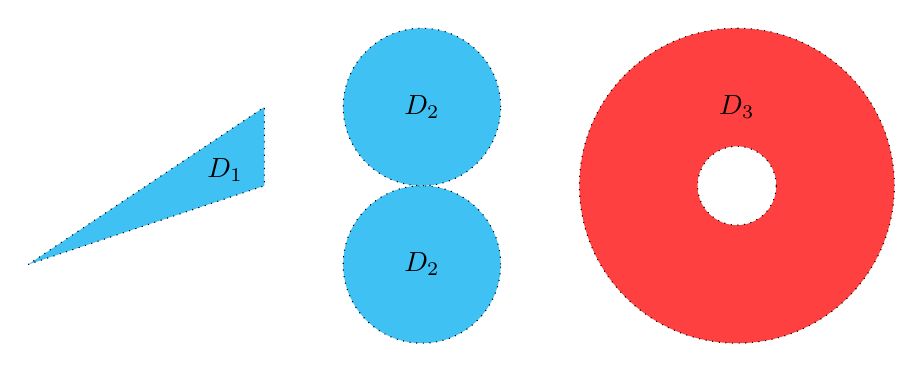
\begin{tikzpicture}
\filldraw[dotted, fill=cyan!75] (-9, 0) -- (-6, 1) -- (-6, 2) -- (-9,0);
\draw (-6.5, 1.2) node{$D_1$};
\filldraw[dotted, fill=cyan!75] (-4, 0) circle (1);
\filldraw[dotted, fill=cyan!75] (-4, 2) circle (1);
\draw (-4, 0) node{$D_2$}; \draw (-4, 2) node{$D_2$};
\filldraw[dotted, fill=red!75] (0,1) circle (2);
\filldraw[dotted, fill=white] (0,1) circle (0.5);
\draw (0, 2) node{$D_3$};
\end{tikzpicture}
\end{center}
From here, we get a theorem similar to Cauchy-Goursat.
\begin{theorem}
If $D$ is simply connected and $C$ is any closed contour in $D$, and if $f$ is analytic on $D$, then $\oint_C f\, dz = 0$.
\end{theorem}

The proof of this can be done by visualizing a domain such as $D_2$, then splitting a contour into its ``simple closed" bits, then applying Cauchy-Goursat. \newpage

\begin{example}
For any closed contour $C$ inside $D: |z|<2$, we have
$$\int_C \frac{\sin z}{(z^2+9)^5} \, dz = 0.$$
\end{example}

The next corollary is particularly powerful.
\begin{corollary}
If $f$ is analytic on a simply connected domain $D$, then $f$ has an antiderivative on $D$. In particular, this implies that entire functions have antiderivatives on all of $\C$.
\end{corollary}
\begin{proof}
Apply Theorem 64.2, so that FTC applies.
\end{proof}

What if we now allow holes in our domains? Consider the \textit{multiply-connected} domain below:
\begin{center}
\includegraphics[scale=0.5]{multiply connected.png}
\end{center}
Notice that we can split our contour $C$ into many pieces, as long as we choose good orientations.
\begin{theorem}
Let $C$, $\{C_k\}_{k=1}^n$ be contours, and assume $f$ is analytic on $C$, all of the $C_k$, and all of the space in between the $C_k$ and $C$. Assume also that the $C_k$ have opposite orientation to $C$. Then
$$\int_C f\, dz + \sum_{k=1}^n \paren{\int_{C_k} f\, dz} = 0.$$
\end{theorem}
\begin{proof}[Proof Sketch for the case above]
Consider the figure above. Now, $\Gamma_1$ and $\Gamma_2$ are obviously simple closed curves, and by construction, $f$ is analytic inside $\Gamma_1$ and $\Gamma_2$, so Cauchy-Goursat applies and
$$\oint_{\Gamma_1} f\, dz + \oint_{\Gamma_2} f\, dz =0+0=0.$$
But staring at the figure for long enough gives that this is the same as saying $\ds\int_C f\, dz + \int_{C_1} f\, dz + \int_{C_2} f\, dz = 0$.
\end{proof}
This gives us the following useful corollary.
\begin{corollary}[Deformation of Paths]
Let $C_1, C_2$ be positively oriented and simple closed contours, and say $C_1$ is interior to $C_2$. If $f$ is analytic on and in between $C_1$ and $C_2$, then
$$\oint_{C_1} f\, dz = \oint_{C_2} f\, dz.$$
\end{corollary}
\begin{example}
Let $C$ be any arbitrary contour exterior to the unit circle. Then $\int_C dz/z = 2\pi i$ by Deformation of Paths.
\end{example}
\subsection*{[54] The Cauchy Integral Formula}
Now, we give an extremely important theorem in complex analysis --- arguably, the rest of this course lies upon this theorem.
\begin{theorem}[Cauchy Integral Formula]
Let $C$ be a simple closed positively-oriented contour, and take $f$ to be analytic on and inside $C$. For any $z_0$ on the interior of $C$, we have
$$\int_C \frac{f(z)}{z-z_0}\, dz = 2\pi i \cdot f(z_0).$$
\end{theorem}
\begin{proof}[Proof Sketch]
Pick $z_0$ inside $C$, and draw a circle $C_\rho$ of radius $\rho$ around $z_0$ and inside $C$. By Deformation of Contours,
$$\int_C \frac{f(z)}{z-z_0}\, dz = \int_{C_\rho} \frac{f(z)}{z-z_0}\, dz.$$
Now, as $z \to z_0$, we can check that
$$\int_{C\rho} \frac{f(z)}{z-z_0}\, dz \to \int_{C\rho} \frac{f(z_0)}{z-z_0}\, dz = f(z_0) \int_{C\rho} \frac{dz}{z-z_0} = 2\pi i f(z_0)$$
by virtue of previous examples.
\end{proof}
This is a dramatic simplification in how certain contour integrals are computed: the type of integral in the Cauchy Integral Formula (CIF) depends only on the function's value at $z_0$.
\begin{example}
Let $C: |z|=1$, positively oriented. Evaluate $\ds\int_C \frac{\cos z}{z(z^2+9)}\, dz$.
\end{example}
\begin{solution}
Write $f(z) := \cos z/(z^2+9)$, so
$$\int_C \frac{\cos z}{z(z^2+9)} = \int_C \frac{f(z)}{z-0}\, dz.$$
Notice that $f$ is analytic on and inside $C$, so the CIF applies and $$\ds\int_C \frac{\cos z}{z(z^2 + 9)}\, dz  =2\pi i \cdot f(0) = \boxed{\frac{2\pi i}9}.$$
\end{solution}
\setcounter{section}{69}
\section{The Generalized CIF and Its Consequences (I)}
The next theorem, as its name suggests, generalizes the CIF. We will see a short proof sketch for the version where $n=1$.

\begin{theorem}[Generalized CIF]
Let $C$ be a simple closed positively-oriented contour, and let $f$ be analytic on and inside $C$. Then for any $z_0$ inside $C$, we have
$$f^{(n)}(z_0) = \frac{n!}{2\pi i}\int_C \frac{f(z)}{(z-z_0)^{n+1}}\, dz.$$
\end{theorem}
Notationally, if $z$ is arbitrary within $C$, we can instead write $\ds \boxed{f^{(n)}(z) = \frac{n!}{2\pi i}\int_C \frac{f(s)\, ds}{(s-z)^{n+1}}}$.

\begin{proof}[Proof Sketch when $n=1$]
From the CIF, we know $f(z) = \ds\frac 1{2\pi i} \int_C \frac{f(s)\, ds}{s-z}$. Now
$$\frac{f(z+\Delta z) - f(z)}{\Delta z} = \frac 1{2\pi i}\int_C \paren{\frac 1{s-z-\Delta z} - \frac 1{s-z}} \frac{f(s)}{\Delta s}\, ds$$
$$=\frac 1{2\pi i}\int_C\brak{\frac 1{(s-z)^2} + \frac{\Delta z}{(s-z-\Delta z)(s-z)^2}} f(s)\, ds.$$
Rearranging, we see that
$$\frac{f(z+\Delta z) - f(z)}{\Delta z} - \frac 1{2\pi i}\int_C \frac{f(s)\, ds}{(s-z)^2} = \frac 1{2\pi i}\int_C \frac{f(s)\Delta z\, ds}{(s-z-\Delta z)(s-z)^2}.$$
Now, $f(s)$ is bounded as it is analytic on and inside $C$, and the denominator $(s-z-\Delta z)(s-z)^2$ approaches $(s-z)^3$ as $\Delta z\to 0$. After some verification of some technicalities, taking the limit as $\Delta z\to 0$ finishes the proof.
\end{proof}
\begin{example}
Let $f(z) := 1$, and pick some $z_0\in\C$. Pick any simple closed positively-oriented contour $C$ around $z_0$. Then
$$\int_C \frac{dz}{z-z_0} = 2\pi i \textsf{ and } \int_C\frac{dz}{(z-z_0)^{n+1}} = 0$$
when $n\geq 1$, as $f'(z) = 0$.
\end{example}
\begin{example}
Let $f(z) := e^{2z}$, and let $C: |z|=1$, positively oriented. Evaluate $\ds\int_C \frac{e^{2z}}{z^3}\, dz$.
\end{example}
\begin{solution}
Using the notation of the Generalized CIF (GCIF), pick $z_0 = 0$ and $n=3-1 = 2$. Then
$$\int_C \frac{e^{2z}\, dz}{z^3} = \int_C \frac{f(z)}{(z-z0)^{2+1}}\, dz,$$
and certainly $f$ is entire and $z_0$ is inside $C$. Hence
$$\int_C \frac{e^{2z}\, dz}{z^3} = f''(0) \cdot \frac{2\pi i}{2!} = 4\cdot \pi i = \boxed{4\pi i}.$$
\end{solution}

The GCIF, in addition to being a powerful computational tool, has many interesting theoretical consequences. We list some of them below.
\newpage
\begin{theorem}
If $f$ is analytic at $z_0\in\C$, then so is $f'$. Hence, $f$ has infinitely many derivatives at $z_0$.
\end{theorem}
\begin{proof}
Saying that $f$ is analytic at a point $z_0$ is the same as saying that $f$ is differentiable in a ball $B(z_0, \epsilon)$, for appropriate $\epsilon > 0$. Pick some simple closed contour $C$ lying in $B(z_0, \epsilon)$, say $C: |z-z_0| < \epsilon/3$, positively-oriented. Then, the GCIF provides a formula for the derivative, so it exists. By induction, $f^{(n)}(z_0)$ exists for all $n\in\N$.
\end{proof}

We have the following corollary, which provides the justification for our proof of Theorem 30.8 earlier in the course.
\begin{corollary}
If $f = u+vi$ is analytic at $z_0 = x_0 + y_0i\in\C$, then all partial derivatives of $u$ and $v$ exist and are continuous at $(x_0, y_0)\in \R^2$.
\end{corollary}

Our next theorem is slightly strange --- it gives a condition for \textit{differentiability} based on integrals.

\begin{theorem}[Morera's Theorem]
Suppose $f$ is continuous on a domain $D\subseteq \C$, and that $\int_C f\, dz = 0$ for all closed contours $C$ inside $D$. Then $f$ is analytic on $D$.
\end{theorem}
\begin{proof}
By FTC, $f$ has an antiderivative $F$ on $D$. But then $F$ is analytic on $D$, as $F' = f$. Applying Theorem 70.4 finishes the proof, as $F'' = f'$ exists.
\end{proof}

Using integration theory, we can in fact go back and estimate derivatives.
\begin{theorem}[Cauchy's Inequality]
Let the circle $C_R: |z-z_0|=R$ be positively oriented, and let $f$ be analytic on and inside $C_R$. If $M_R := \max\set{|f(z)|: z\in C_R}$, then
$$\abs{f^{(n)}(z_0)} = \frac{n!M_R}{R^n}.$$
\end{theorem}
\begin{proof}
By the GCIF, we know that $\ds f^{(n)}(z_0) = \frac{n!}{2\pi i}\int_{C_R} \frac{f(z)\, dz}{(z-z_0)^{n+1}}$. Using this and the Estimation Lemma, we have
$$\abs{f^{(n)}(z_0)} = \frac{n!}{2\pi}\abs{ \int_{C_R} \frac{f(z)\, dz}{(z-z_0)^{n+1}}} \leq \frac{n!}{2\pi} \cdot \frac{M_R}{R^{n+1}} \cdot 2\pi R = \frac{n!M_R}{R^n},$$
which completes the proof.
\end{proof}

\setcounter{section}{73}
\section{The Generalized CIF and Its Consequences (II)}
The Generalized CIF also gives us the following powerful result, which is obviously false in real analysis.
\begin{theorem}[Liouville's Theorem]
If $f$ is entire and bounded, then $f$ is constant.
\end{theorem}
\begin{proof}
Take some $R>0$ and $z_0\in\C$. Say that $f$ is entire and bounded by $M>0$; i.e., $|f(z)| \leq M$ for all $z\in\C$. Then, Cauchy's Inequality applies and for a circle $C_R$ and $M_R$ as in that theorem,
$$0\leq \abs{f'(z_0)} = \frac{M_R}R \leq \frac MR \to 0$$
as $R\to \infty$. Hence $f'(z_0) = 0$, so $f$ is constant.
\end{proof}

This allows us an easy proof of the algebraic closure of $\C$. Note that this statement is neither fundamental, nor algebraic. \newpage
\begin{theorem}[Fundamental Theorem of Algebra]
Let $p(z) = a_0 + a_1z + \cdots + a_nz^n\in\C[z]$, with $a_n\neq 0$, $n\geq 1$. Then $p$ has a root in $\C$. Equivalently, $\C$ is algebraically closed.
\end{theorem}
\begin{proof}
Assume for contradiction that $p$ does not have a root in $\C$. Then $f(z) := 1/p(z)$ is entire, and Theorem 13.6 provides a bound as follows: there exists an $R>0$ such that for all $|z|>R$, we have
$$|f(z)| = \abs{\frac 1{p(z)}} < \frac 2{|a_n|R^n}.$$
This shows that $f$ is bounded outside of the circle $|z|=R$. But the interior of the circle is closed, so $f$ is bounded there, say by some $M_0>0$. Take $M$ to be the maximum of the two bounds, so $f$ is bounded everywhere and entire, so $f$ is constant. Hence $p$ is constant, but we assumed otherwise --- a contradiction.
\end{proof}
\subsection*{[59] The Maximum Modulus Principle}
The (regular) CIF has this important consequence, which saves us work if we ever have to do an optimization problem.
\begin{theorem}[Maximum Modulus Principle]
Let $D\subseteq\C$ be a domain (which is open), and let $f$ be a nonconstant analytic function on $D$. Then $|f(z)|$ has no maximum on $D$.
\end{theorem}

We first state and prove a simpler version of the Maximum Modulus Principle (MMP) for circles.
\begin{lemma}[MMP for Disks]
Let $f$ be analytic on $B(z_0, \epsilon)$, for some $z_0\in\C$ and $\epsilon>0$. Suppose $|f(z)| \leq |f(z_0)|$ for every $z\in B(z_0, \epsilon)$. Then $f$ is constant on $B(z_0,\epsilon)$.
\end{lemma}
\begin{proof}
Pick an arbitrary $z_1\in B(z_0, \epsilon)$. We show that $|f(z_0)| = |f(z_1)|$, so that Proposition 30.9 finishes the proof. Take $\rho:= |z_1 - z_0|$, and define $C_\rho: |z-z_0| = \rho$, positively-oriented. Then $C_\rho$ is a circle centered at $z_0$, passing through $z_1$, lying entirely in $B(z_0, \epsilon)$. By the CIF, we see that after parameterizing $C_\rho$ in the obvious way,
$$f(z_0) = \frac 1{2\pi i}\int_{C_\rho} \frac{f(z)\, dz}{z-z_0} \implies f(z_0) = \frac 1{2\pi i}\int_0^{2\pi} \frac{f(z_0 + \rho e^{i\theta})}{\rho e^{i\theta}} \cdot \rho ie^{i \theta}\, d\theta,$$
which simplifies further to $\ds f(z_0) = \frac 1{2\pi} \int_0^{2\pi} f(z_0+\rho e^{i\theta})\, d\theta$. By our assumption, we have
$$|f(z_0)| \leq \frac 1{2\pi}\int_0^{2\pi} |f(z_0 + \rho e^{i\theta})|\, d\theta \leq \frac 1{2\pi}\int_0^{2\pi} |f(z_0)|\, d\theta,$$
but we know that $\ds\frac 1{2\pi}\int_0^{2\pi} |f(z_0)|\, d\theta = |f(z_0)|$, hence the inequalities above are actually equalities and we write
$$|f(z_0)| = \frac 1{2\pi}\int_0^{2\pi} |f(z_0)| \, d\theta = \frac 1{2\pi}\int_0^{2\pi} \abs{f(z_0 + \rho e^{i\theta})}\, d\theta$$
$$\implies \int_0^{2\pi} \brak{\abs{f(z_0)} - \abs{f(z_0 + \rho e^{i\theta})}}\, d\theta = 0.$$
The integrand of the above is continuous and nonnegative, so $|f(z_0)| = \abs{f(z_0 = \rho e^{i\theta})}$. Since $z_1$ lies on $C_\rho$, we have $|f(z_0)| = |f(z_1)|$.
\end{proof}
\newpage
\setcounter{section}{77}
\section{The MMP, Sequences and Series}
\subsection*{[59] The Maximum Modulus Principle}
Continuing on, we now prove Theorem 74.3.
\begin{proof}[Proof of Thm. 74.3]
We prove by contrapositive. Take some $z_0\in D$ such that $|f(z)| \leq |f(z_0)|$. Since $D$ is connected, draw a piecewise linear curve $\gamma$ between $z_0$ and any point $p\in D$. Picking appropriate points $z_j$ along $\gamma$ with $p = z_n$, draw balls of radius $\delta$ within $D$, such that $B(z_j, \delta) \cap B(z_{j+1}, \delta)\neq \varnothing$ and each $B(z_j, \delta)$ is contained in $D$. Apply Lemma 74.4 along each point to see that $f(z_0) = f(z_1) = \cdots = f(z_n) = f(p)$, so $f$ is constant.
\end{proof}

From here, we get the following corollary.
\begin{corollary}
Let $R\subseteq \C$ be a closed bounded region, and let $f$ be non-constant and analytic on the interior of $R$ as well as continuous on $\del R$. Then $f$ attains its maximum on $\del R$.
\end{corollary}

Additionally, if $f = u+vi$, then $u$ has a maximum on $\del R$, and never on the interior of $R$. To see this, let $g := \exp f$, and apply the corollary. We should notice the asymmetry between maximums and minimums here: we know that $f(z) = z^2$ attains its minimum \textit{within} the region $R = \{|z| \leq 1\}$, and not on the boundary.

\subsection*{[60]/[61] Sequences and Series}
We now take a short break to discuss sequences and series, which will return powerfully once we begin discussing integrals again. Most of this section is review or at least intuitive.
\begin{definition}
A sequence $(z_n)$ of complex numbers \textit{converges to $z\in \C$} if for every $\epsilon > 0$, there exists an $N\in\N$ such that for all $n>N$, we have $|z_n - z| < \epsilon$. If such a $z$ exists, then we say that $z$ is the \textit{limit} of the sequence and write $\lim z_n = z$.
\end{definition}

Of course, the limit of a sequence is \textit{unique} when it exists. If no such limit exists, we say that the sequence \textit{diverges}.
\begin{theorem}
Let $z_n = x_n + y_ni$, and $z=x+yi\in\C$. Then $(z_n)\to z$ if and only if we have both $(x_n) \to x$ and $(y_n)\to y$.
\end{theorem}
This is not too surprising: a complex sequence can be considered a pair of real sequences.
\begin{example}
Let $z_n = \ds 5 + \frac{(-1)^ni}n$. Then $x_n = 5\to 5$ and $y_n = \ds\frac{(-1)^n}n\to 0$, so $z_n\to 5+0i = 5$.
\end{example}
\begin{example}
Let $z_n = -1 - \ds\frac i{n^2}$. Then $z_n\to -1$, but if we write
$$r_n = |z_n| = \sqrt{1+n^{-4}} \to 1 = r = |x_n|, \textsf{ and}$$
$$\Arg(z_n)\to -\pi,$$
we see that the polar analogue of Theorem 78.3 does not work.
\end{example}
We move on to discussing series.
\begin{definition}
Let $(z_n)$ be a sequence in $\C$. We define the \textit{infinite series} by
$$\sum_{n=0}^\infty z_n := \lim_{n\to\infty} \sum_{j=0}^n z_j,$$
whenever this limit exists.
\end{definition}
Of course, complex series can be split into a pair of real series in the obvious way.
\begin{theorem}
Let $(z_n)$ be a sequence, $z_n = x_n + y_ni$, and $z = x+yi\in C$. Then $\sum z_n = z$ if and only if we have both $\sum x_n = x$ and $\sum y_n =y$.
\end{theorem}
The $n$th term test still holds from real analysis.
\begin{corollary}[$n$th Term Test]
If $\sum z_n$ converges, then $\lim z_n = 0$.
\end{corollary}

We also have the notion of \textit{absolute convergence}:
\begin{definition}
We say that $\sum z_n$ \textit{converges absolutely} if $\sum |z_n|$ converges.
\end{definition}
Of course, it goes without saying that if $\sum |z_n|$ converges, so does $\sum z_n$.
\vspace{0.2 cm}

Complex power series are defined in the same way.
\begin{definition}
A \textit{power series} is a function
$$f(z) := \sum_{n=0}^\infty a_n(z-z_0)^n,$$
for fixed $a_n, z_0\in\C$, whenever the sum converges.
\end{definition}
\setcounter{section}{79}
\section{Taylor and Laurent Series (I)}
Let us view an example of a familiar power series.
\begin{example}
Let $f(z) = \sum z^n$. Then $f(z) = 1/(1-z)$ whenever $|z|<1$, as
$$\sum_{n=0}^N z^n = \frac{1-z^{N+1}}{1-z}; \textsf{ hence}$$
$$\frac 1{1-z} - \sum_{n=0}^N z^n = \frac{z^{N+1}}{1-z}\to 0$$
if $|z|<1$. If $|z|\geq 1$, the sum diverges as usual.
\end{example}
The following theorem should be familiar to us.
\begin{theorem}[Taylor's Theorem]
Let $f$ be analytic on some $B(z_0, R_0)$. Then $f(z) = \sum a_n(z-z_0)^n$ for all $z\in B(z_0, R_0)$, where $a_n = f^{(n)}(z_0)/n!$. 
\end{theorem}
Since Taylor series are differentiable, we see that a function is analytic in some ball if and only if it can be expanded as a Taylor series in that ball. In particular, if $f$ is entire, then it has a Taylor series expansion everywhere.

For a proof of Taylor's Theorem, see [63] in the text. We view an example. \newpage
\begin{example}
Let $f(z) = 1/(1-z)$, and $z_0=  i$. Note that $f$ is analytic on $B(i, \sqrt 2)$, so Taylor's Theorem guarantees a power series representation on that ball. Write
$$\frac 1{1-z} = \frac 1{1-i-(z-i)} = \frac 1{1 - (z-i)/(1-i)} \cdot \frac 1{1-i}.$$
Now, whenever $z\in B(i, \sqrt 2)$, we observe that this implies $|(z-i)/(1-i)| < 1$, so we can write
$$\frac 1{1 - (z-i)/(1-i)} \cdot \frac 1{1-i}. = \frac 1{1-i}\sum_{n=0}^\infty \paren{\frac{z-i}{1-i}}^n$$
on that ball. We can simplify this as we wish: $\ds\frac 1{1-z} = \boxed{\sum_{n=0}^\infty \frac 1{(1-i)^{n+1}}(z-i)^n}$ for all $z\in B(i, \sqrt 2)$.
\end{example}

Now, we turn our attention to a phenomenon that occurs rather exclusively to complex functions: we can have negative powers in our ``power series" representations.
\begin{example}
Let $f(z) = e^{-z}/z^2$. Then $f$ is certainly not analytic at $z=0$, but
$$f(z) = \frac 1{z^2}\sum_{n=0}^\infty \frac{(-z)^n}{n!} = \frac 1{z^2} - \frac 1z + \frac 12 - \frac z6 + \frac{z^2}{24}-\cdots, \,\, (z\neq 0),$$
which is a ``power series" save for the negative powers $-2$ and $-1$ appearing.
\end{example}
\begin{example}
Let $f(z) = \ds \frac{1+2z^2}{z^3+z^5}$. Then $f$ is not analytic at $z = 0, \pm i$. But for $0< |z|< 1$, we can safely write
$$f(z) = \frac{1+2z^2}{z^3(1+z^2)} = \frac 1{z^3} \paren{2 - \frac 1{1+z^2}} = \frac 1{z^3}\paren{2 - \sum_{n=0}^\infty (-1)^nz^{2n}}$$
$$\implies f(z) = \frac 1{z^3} + \frac 1z - z + z^3 - \cdots, \,\, (0 < |z| < 1),$$
where the negative powers $-3$ and $-1$ appear.
\end{example}
This is the idea of a \textit{Laurent series}, which we introduce below.
\begin{theorem}[Laurent's Theorem]
Let $f$ be analytic on some \textit{annulus} $R_1 < |z-z_0| < R_2$, and let $C$ be a positively oriented, simple closed contour on the annulus. If
$$a_n = \frac 1{2\pi i}\int_C \frac{f(z)\, dz}{(z -z_0)^{n+1}}, \,\, n\geq 0 \textrm{ and}$$
$$b_n = \frac 1{2\pi i}\int_C \frac{f(z)\, dz}{(z - z_0)^{-n+1}}, \,\, n\geq 1,$$
then
$$f(z) = \sum_{n=0}^\infty a_n(z-z_0)^n + \sum_{n=1}^\infty \frac{b_n}{(z-z_0)^n}$$
on the annulus. Alternatively, we can write $\ds c_n = \frac 1{2\pi i}\int_C \frac{f(z)\, dz}{(z-z_0)^{n+1}}$ for all $n\in\Z$, so that
$$f(z) = \sum_{n=-\infty}^\infty c_n(z-z_0)^n.$$
\end{theorem}
\newpage
\setcounter{section}{82}
\section{Taylor and Laurent Series (II)}
In this section, we view examples of Taylor and Laurent series.
\begin{example}
Let $f(z) := \sin z$, and $z_0 = \pi/2$. Find the Taylor series of $f$ centered at $z_0$.
\end{example}
\begin{solution}
Notice that $\sin z = \cos(z-\pi/2)$. Then we can just use the Taylor series for cosine:
$$\sin z = \cos(z-\pi/2) = 1 - \frac{(z-\pi/2)^2}{2!} + \frac{(z-\pi/2)^4}{4!} - \cdots = \boxed{\sum_{n=0}^\infty (-1)^n \frac{(z-\pi/2) ^{2n}}{(2n)!}}.$$
This example illustrates an important point: apply shifts before resorting to computation of derivatives.
\end{solution}
\begin{example}
Let $f(z) = z/(z^4+4)$. Find the \textit{Maclaurin series} of $f$.
\end{example}
\begin{solution}
Certainly, $f$ is analytic at $0$, so the Maclaurin series exists. Using some algebra, we write
$$f(z) = z\cdot \frac 1{z^4+4} = z\paren{\frac 1{1 + \frac{z^4}4}}\cdot \frac 14 = \frac z4\paren{\frac 1{1 + \frac{z^4}4}}.$$
Now
$$\frac 1{1 + \frac{z^4}4} = 1 + \paren{-\frac{z^4}4} + \paren{-\frac{z^4}4}^2 + \cdots = 1- \frac{z^4}4 + \frac{z^8}{16} - \frac{z^{12}}{64} + \cdots,$$
whenever $|z^4/4|< 1 \implies |z|<\sqrt 2$. Hence we have the following series for $f$, valid whenever $|z|<\sqrt 2$:
$$f(z) = \frac 14\paren{z - \frac{z^5}4 + \frac{z^9}{16} - \frac{z^{13}}{64} + \cdots} = \boxed{ \sum_{n=0}^ \infty (-1)^n\frac{z^{4n+1}}{4^{n+1}}}.$$
\end{solution}
\begin{example}
Find the Laurent series for $f(z) = e^z/z^3$, centered at $z_0 = 0$.
\end{example}
\begin{solution}
Notice that $f$ is not analytic at $z_0=0$, but definitely whenever $0 < |z| < \infty$, so a Laurent series exists. Now
$$f(z) = \frac 1{z^3}e^z = z^{-3}\paren{1 + z + \frac{z^2}{2!} + \frac{z^3}{3!}+\cdots} = \boxed{\sum_{n=-3}^\infty \frac{z^n}{(n+3)!}},$$
provided that $z\neq 0$.
\end{solution}
\begin{example}
Find the Laurent series for $f(z):= z/(z+1)^3$, centered at $z_0 = -1$.
\end{example}
\begin{solution}
We compute from definition here. The coefficients $c_n$ for the Laurent series are given by
$$c_n = \frac 1{2\pi i}\int_C \frac{z/(z+1)^3}{(z + 1)^{n+1}}\, dz= \frac 1{2\pi i}\int_C \frac{z\, dz}{(z+1)^{n+4}},$$
where $C$ is any contour with $z=-1$ in its interior. By the GCIF, if we let $g(z) = z$, we see that $g^{(n+3)}(-1)/n! = c_n$, so that $c_{-2} = 1$, $c_{-3} = -1$, and $c_n = 0$ otherwise. Thus, our Laurent series is in fact finite:
$$f(z) = \boxed{\frac 1{(z+1)^2} - \frac 1{(z + 1)^3}},$$
provided that $z\neq -1$. Notice that this is just the partial fraction decomposition of $f$, which is not surprising: just as polynomials have finite Taylor expansions everywhere, rational functions should have finite Laurent expansions on their domains.
\end{solution}
We finally comment that if $f$ is analytic at $z_0$, the Laurent series expansion coincides with the Taylor series, and no negative terms are generated.

\setcounter{section}{89}
\section{Laurent Series, Singularities, and Residues}
We view two more applications of Laurent series.
\begin{example}
Let $f(z) := (z+1)/(z-1)$, and let $z_0 := 0$. Consider the open disk $B(z_0, 1) = B(0, 1)$. Then $f$ is analytic there, and we have the Taylor series
$$\frac{z+1}{z-1} = (z+1)\brak{-\sum_{n=0}^\infty z^n} = -1 - 2\sum_{n=1}^\infty z^n.$$
[We could have done this by writing $f(z) = 1 + 2/(z-1)$ as well.] Additionally, $f$ is analytic whenever $|z|>1 \iff |1/z|<1$. Hence, we get a Laurent series on the annulus $1 < |z| < \infty$:
$$f(z) = \frac{z+1}{z-1} = \frac{1+1/z}{1-1/z} = \paren{1 + \frac 1z}\sum_{n=0}^\infty \paren{\frac 1z}^n,\,\, |z|>1.$$
Expanding this gives
$$f(z) = \sum_{n=0}^\infty \paren{\frac1z}^n + \sum_{n=0}^\infty \paren{\frac1z}^{n+1} = 1 + 2\sum_{n=1}^\infty \paren{\frac 1z}^n.$$
\end{example}
\begin{example}
We claim that $\int_C e^{1/z}\,dz = 2\pi i$ for any positively oriented closed contour $C$ around $0$. To see this, we write the Laurent expansion for $e^{1/z}$ for $z\neq 0$: $e^{1/z} = \sum_{n=0}^\infty z^{-n}/n!$. Notice that if $f(z) = e^{1/z}$, then from definition of the coefficients
$$c_{-1} = \frac 11 = 1 = \frac 1{2\pi i}\int_C f(z)\, dz = \frac 1{2\pi i}\int_C e^{1/z}\, dz,$$
so solving for the integral proves our claim.
\end{example}
\subsection*{[74] Singularities}
The above example is particularly useful: it gave us the answer to an integral because we knew a function's Laurent series. Recall that Laurent series only have negative powered terms around some annulus, centered at a non-analytic point. This is the topic of study in this section.
\begin{definition}
Let $f$ be a function. We say that $z_0\in\C$ is a \textit{singularity of $f$} if $f$ is not analytic at $z_0$, but analytic at points arbitrarily close to $z_0$. A singular point of $f$ is an \textit{isolated singularity} if $f$ is analytic on $D(z_0, \epsilon)$ for some $\epsilon>0$.
\end{definition}
\newpage

\begin{example}
Let $f(z) = \ds\frac{z-1}{z^5(z^2+9)}$. Then $f$ has exactly $3$ singularities: $z = 0, \pm 3i$, and all of these are isolated, as $f$ is analytic on the punctured balls $D(0, 1)$, $D(3i, 1)$, and $D(-3i, 1)$.
\end{example}
\begin{example}
Let $f(z) = \Log z$. Then $f$ has singularities along the entire negative real axis due to a branch cut. These are \textit{not} isolated.
\end{example}
\begin{example}
Let $f(z) = \csc\paren{\frac \pi2}$. Then $f$ has singularities at all $z = 0, 1/n$ for $n\in\N$. The singularities $z=1/n$ are isolated, but the singularity $z=0$ is not:
\begin{center}
\begin{tikzpicture}
\draw (0, -1) -- (0, 1);
\draw (-0.2, 0) -- (3.4, 0);
\filldraw[color=red!75, fill=red!75] (2,0) circle (0.03);
\filldraw[color=red!75, fill=red!75] (2/2, 0) circle (0.03);
\filldraw[color=red!75, fill=red!75] (2/3, 0) circle (0.03);
\filldraw[color=red!75, fill=red!75] (2/4, 0) circle (0.03);
\filldraw[color=red!75, fill=red!75] (2/5, 0) circle (0.03);
\draw[color=red!75] (0,0) -- (2/5,0);
\filldraw[color=green!75, fill=green!75] (0,0) circle (0.03);
\draw (2,0) node[anchor=north]{$1$};
\draw[dotted] (2,0) circle (0.75);
\draw[dotted] (2/2,0) circle (0.75/4);
\draw[dotted] (2/3,0) circle (0.75/8);
\end{tikzpicture}
\end{center}
\end{example}
We remark that if $C$ is a simple closed contour, and $f$ is analytic inside $C$ except for finitely many points $z_j$, then all of the $z_j$ are isolated. Now, consider one isolated singularity $z_0$ of $f$. This means we can take some $R>0$ such that $f$ is analytic on $0 < |z-z_0| < R$, so we have a Laurent series expansion in that region. We make the following definition.
\begin{definition}
If $z_0\in\C$ is an isolated singularity of $f$, we define the \textit{residue} of $f$ at $z_0$ by
$$\Res_{z=z_0} f(z) := c_{-1} = \frac 1{2\pi i} \int_C f(z)\, dz,$$
where $c_{-1}$ is the coefficient of the $1/(z-z_0)$ term in the Laurent series expansion that occurs centered at $z_0$.
\end{definition}
This gives us a fast way to compute integrals, like we have seen before: just find the residue.
\setcounter{section}{92}
\section{More Examples, Calculus with Power Series}
[This discussion section just had more helpful examples.]
\begin{example}
Find the Laurent series for $f(z) := z^2\sin(1/z^2 )$ on the region $0<|z|<\infty$.
\end{example}
\begin{solution}
When $z\neq 0$, we may write
$$\sin\paren{\frac 1{z^2}} - \frac 1{z^2} - \frac{(1/z^2)^3}{3!} + \frac{(1/z^2)^5}{5!} - \cdots = z^{-2} - \frac{z^{-6}}{3!} + \frac{z^{-10} }{5!} - \cdots,$$
so that
$$f(z) = z^0 - \frac{z^{-4}}{3!} + \frac{z^{-8}} {5!} - \cdots = \boxed{\sum_{k=0}^\infty \frac 1{z^{4k}} \frac{(-1)^k}{(2k+1)!}}.$$
\end{solution}
\begin{example}
Find the Laurent series for $g(z) := a/(z-a)$, on $|a| < |z| < \infty$.
\end{example}
\begin{solution}
Notice that when $|z| > |a|$, we have $|1/z| < |1/a|$ as we are comparing positive real numbers. Write
$$g(z) = \frac a{z-1} = \frac{a/z}{1-a/z},$$
which is analytic whenever $z\neq a$. Now when $|1/z| < |1/a|$, we have \newpage
$$g(z) = \frac az\paren{\frac 1{1-a/z}} = \frac az\paren{1 + \frac az + \frac{a^2}{z^2}+\cdots} = \boxed{\sum_{k=0}^\infty \paren{\frac az}^{k+1}}.$$
\end{solution}
As in real analysis, complex power series may be differentiated and integrated term by term.
\begin{theorem}
A power series $S(z) := \sum a_n(z-z_0)^n$ defines an analytic function in its circle of convergence. In particular, $S$ can be differentiated term by term:
$$\frac d{dz}\sum_{n=0}^\infty a_n(z-z_0)^n = \sum_{n=0}^\infty \frac d{dz}[a_n(z-z_0)^n],$$
and if $C$ is any contour lying within the circle of convergence of $S$, then the contour integral can be done term by term:
$$\int_C \paren{\sum_{n=0}^\infty a_n(z-z_0)^n}\, dz = \sum_{n=0}^\infty\paren{\int_C a_n(z-z_0)^n \, dz}.$$
\end{theorem}
\section{Residues and Poles}
We view an example of calculating a residue to solve an integral.
\begin{example}
Let $C: |z|=1$, positively oriented. Find $\ds\int_C \frac{e^z-1}{z^4}\, dz$.
\end{example}
\begin{solution}
Let $f(z) := (e^z-1)/z^4$. Then $f$ is analytic on $0 < |z| < \infty$, so it has a Laurent series expansion there:
$$\frac{e^z-1}{z^4} = \frac 1{z^4}\sum_{n=1}^\infty \frac{z^n}{n!} = \sum_{n=1}^\infty \frac{z^{n-4}}{n!}.$$
The residue of $f(z)$ is the $z^{-1}$ coefficient: $z^{3-4}/3! = z/6$. Hence
$$\int_C f(z)\, dz = 2\pi i \Res_{z=0} f(z) = 2\pi i\cdot\frac 16 = \boxed{\frac{\pi i}3}.$$
\end{solution}
This example is in fact an indication of a more general statement.
\begin{theorem}[Cauchy's Residue Theorem]
Let $C$ be a positively-oriented simple closed contour, and let $f$ be analytic on and inside $C$, except for finitely many $\{z_j\}_{j=1}^n$, which are isolated singularities. Then
$$\int_C f(z)\, dz = 2\pi i \sum_{j=1}^n \Res_{z= z_j} f(z).$$
\end{theorem}
\begin{proof}
Inside $C$, draw non-overlapping balls $B(z_j, \delta_j)$ around each $z_j$, and let the $C_j$ be the boundary of each ball, positively oriented. By Theorem 64.5 (and taking care of the signs), we see that
$$\int_C f\, dz - \sum_{j=1}^n\int_{C_j} f\, dz = 0.$$
\newpage
But by definition $\ds\int_{C_j} f\, dz = 2\pi i\Res_{z = z_j} f(z)$, so this completes the proof.
\end{proof}
\begin{example}
Find $\ds\int_C \frac{4z-5}{z(z-1)}\, dz$, where $C: |z|=2$, positively oriented.
\end{example}
\begin{solution}
Letting $f(z) = 4z-5/(z(z-1))$, we have two isolated singularities inside $C$, namely $z=0$ and $z=1$. At $z=0$, we can write
$$f(z) =  -\frac{4z-5}{z} \cdot \frac 1{1-z} = -\paren{4 - \frac 5z}\sum_{n=0}^\infty z^n,\,\, 0 < |z| < 1.$$
By inspection, we read off the residue: $\ds\Res_{ z=0} f(z) = 5$. Similarly, when $z=1$, note that
$$\frac 1z= \frac 1{1+(z-1)} = \sum_{n=0}^\infty (-1)^n(z-1)^n,\,\, |z-1|<1.$$
Hence
$$f(z) = \frac 1{z-1}(4z-5)\sum_{n=0}^\infty (-1)^n (z-1)^n = \paren{4 - \frac 1{z-1}}\sum_{n=0}^\infty (-1)^n(z-1)^n, \,\, 0 < |z-1| < 1,$$
so we read off the residue again: $\ds\Res_{z=1} f(z) = -1$. By Cauchy's Residue Theorem, we have $\ds\int_C f(z)\, dz = 2\pi i(5-1) = \boxed{8\pi i}$.
\end{solution}

We should note that not all singularities have meaningful residues. In this course, we will distinguish three types of singularities, but will focus only on one.
\begin{definition}
Let $z_0\in\C$ be a singularity of $f$. If the Laurent coefficients $c_k$ satisfy $c_k = 0$ for all $k < 0$, then $z_0$ is a \textit{removable singularity} of $f$.
\end{definition}
\begin{example}
Let $f(z):= (1-\cos z)/z^2$. Then $f$ has an isolated singularity at $z_0 = 0$ but when $z\neq 0$, $f$ has the Laurent series expansion
$$f(z) = \frac 12 - \frac{z^2}{4!} + \frac{z^4}{6!} - \cdots,$$
which has no negative terms. We can ``patch" the singularity by extending $f(0) = 1/2$, and then $f$ would in fact be an entire function.
\end{example}
We can consider the opposite extreme, though we will not see examples.
\begin{definition}
Let $z_0\in\C$ be a singularity of $f$. If infinitely many of the $c_k$ are nonzero when $k<0$, then $z_0$ is an \textit{essential singularity} of $f$.
\end{definition}
Finally, we consider the ``usual" case.
\begin{definition}
Let $z_0\in\C$ be a singularity of $f$. If only finitely many of the $c_k$ are nonzero when $k<0$, then $z_0$ is a \textit{pole}. The \textit{order} of the pole is the ``last" $k$ where $c_k$ is nonzero: i.e., it is the integer $m>0$ such that $c_{-m} \neq 0$ but $c_{-n} - 0$ for all $n > m$. In the case that $m=1$, we say that $z_0$ is a \textit{simple pole}.
\end{definition}
\setcounter{section}{97}
\newpage
\section{Residues at Poles}
When we know that a singular point is a pole, we can calculate its residue easily.
\begin{theorem}
Suppose that $f$ has an isolated singularity at $z_0\in \C$. Then $z_0$ is a pole of order $m$ if and only if $f(z) = \phi(z)/(z-z_0)^m$, where $\phi$ is analytic and nonzero at $z_0$. If this is the case, then
$$\Res_{z=z_0} f(z) = \frac{\phi^{(m-1)}(z_0)}{(m - 1)!}.$$
\end{theorem}
\begin{example}
Let $f(z) = \ds\frac{z+4}{z^2+1}$. Then $f$ has singularities at $\pm i$. At $z=i$, we write
$$f(z) = \frac 1{z-i} \cdot \frac{z+4}{z+i} =: \frac 1{z-1}\phi(z).$$
We check that $\phi$ is analytic and nonzero at $i$, so $\ds\Res_{z=i} f(z) = \phi(i) = \boxed{\frac{i+4}{2i}}.$
\end{example}

We also define the dual notion: a \textit{zero} of order $m$.
\begin{definition}
Suppose $f$ is analytic at $z_0$. We say that $f$ has a \textit{zero of order $m$} at $z_0$ if $f(z_0) = f'(z_0) = \cdots = f^{(m-1)}(z_0) = 0$, but $f^{(m)}(z_0) \neq 0$.
\end{definition}
\begin{theorem}[Factorization Theorem]
Suppose $f$ is analytic at $z_0$. Then $z_0$ is a zero of order $m$ if and only if $f(z) = (z-z_0)^m g(z)$, where $g$ is analytic and nonzero at $z_0$.
\end{theorem}

The next theorem states that zeros become poles when placed in the denominator.
\begin{theorem}
Suppose $p, q$ are analytic at $z_0$, $p(z_0) \neq 0$, and $q$ has a zero of order $m$ at $z_0$. Then $p/q$ has a pole of order $m$ at $z_0$.
\end{theorem}
\begin{proof}
Applying Theorem 98.4, write $p/q = p/((z-z_0)^mg)$, where $g$ is analytic and nonzero at $z_0$. By Theorem 98.1, write $\phi := p/g$, so $p/q = \phi/ (z-z_0)^m$. Now $\phi(z_0) \neq 0$ and $\phi$ is analytic at $z_0$ since $p$ and $g$ are analytic at $z_0$. Hence $z_0$ is a pole of order $m$.
\end{proof}
\begin{example}
Let $f(z) := 1/(1-\cos z)$. Then $p(z) = 1$ and $q(z) = 1-\cos z$. Fix $z_0 = 0$. Then $q(0) = q'(0) = 0$, but we verify $q''(0) = \cos 0 = 1\neq 0$. Hence, $z_0$ is a zero of order $2$ of $q$, so it is a pole of order $2$ of $f$.
\end{example}
The next theorem simplifies our calculations when a pole is simple.
\begin{theorem}
Let $p,q$ be analytic at $z_0$, $p(z_0)\neq 0$, and $z_0$ be a simple zero of $q$: i.e., $q(z_0) = 0$ and $q'(z_0)\neq 0$. Then $p/q$ has a simple pole at $z_0$, and the residue is given by
$$\Res_{z=z_0} \frac pq = \frac{p(z_0)}{q'(z_0)}.$$
\end{theorem}
\begin{proof}
Write $p/q = p/[(z-z_0)g] = \phi/(z-z_0)$ as before. By Theorem 98.1, we have $\ds\Res_{z=z_0} p/q = \phi(z_0)$, so that $\phi(z_0) = p(z_0)/g(z_0)$. The product rule shows that $q' = (z-z_0)g' + g$, so $q'(z_0) = g(z_0)$. 
\end{proof}
We now view some examples. \newpage
\begin{example}
Let $f(z) := \cot z = \cos z/\sin z$. Notice that $\sin z$ has simple zeros at $n\pi$, $n\in\Z$, so Theorem 98.7 tells us that $\cot z$ has simple poles at $n\pi$, and
$$\Res_{z=n\pi} \cot z = \frac{\cos(n\pi)}{\cos(n\pi )} = \boxed 1.$$
\end{example}
\begin{example}
Let $f(z) = z/(z^4+4)$. Then $z^4+4$ has a simple zero at $z_0 = 1+i$, so $z_0$ is a simple pole of $f$. Hence
$$\Res_{z=1+i} \frac z{z^4+4} = \frac{z_0}{4z_0^3} = \boxed{-\frac i8}.$$
\end{example}
\setcounter{section}{99}
\section{Improper Real Integrals}
Recall that if $f: [0, \infty)\to \R$ is continuous, we define $\ds\int_0^\infty f(x)\, dx := \lim_{t\to \infty} \int_0^t f(x)\, dx$, whenever the limit exists. Similarly, if $f: \R\to \R$ is continuous, we define by ``splitting" the integral
$$\int_{-\infty}^\infty f(x)\, dx := \lim_{s\to\infty}\int_{-s}^0 f(x) \, dx + \lim_{t \to\infty} \int_0^t f(x)\, dx.$$
But this is not the only way to define an integral across the real line.
\begin{definition}
Let $f: \R\to\R$ be continuous. We define the \textit{Cauchy principal value} by
$$\PV\int_\R f(x)\, dx := \lim_{t\to\infty} \int_{-t}^t f(x)\, dx.$$
\end{definition}
\begin{lemma}
If $\int_\R f(x)\, dx$ exists, then $\PV \int_\R f(x)\, dx = \int_\R f(x)\, dx$.
\end{lemma}
Hence, the principal value agrees with the standard integral whenever the standard integral exists. However, the converse is not always true.
\begin{example}
Clearly, $\int_{-t}^t x\, dx = 0$, so $\PV\int_\R x\,dx = 0$. But $\int_\R x\, dx$ diverges.
\end{example}
However, the converse holds if $f$ is even:
\begin{proposition}
Let $f$ be even. Then $\int_\R f(x)\, dx = \PV \int_\R f(x)\, dx$, provided that the standard integral exists.
\end{proposition}
\begin{proof}
Since $f$ is even, we have $\int_0^t f(x)\, dx = \frac 12\int_{-t}^t f(x)\, dx$, so as $t\to \infty$, we observe that
$$\int_0^t f(x)\, dx = \frac 12\PV \int_\R f(x)\, dx.$$
Doubling finishes the proof.
\end{proof}

We now show how to calculate $\PV\int_\R f(x)\, dx$ in a special case.
\begin{example}
Find $\ds\int_\R \frac{dx}{x^6+1}$.
\end{example}
\begin{solution}
Let $f(x) = 1/(x^6+1)$. Notice that $x^6+1$ only has complex roots, and we consider the ones with positive imaginary part: \newpage
\begin{center}
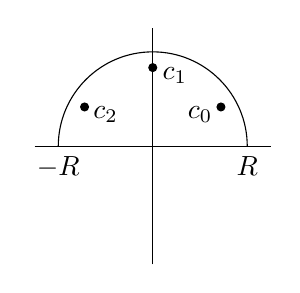
\begin{tikzpicture}
\filldraw (0,1) circle (0.05);
\filldraw (0,0.9) node[anchor=west]{$c_1$};
\filldraw (0.6, 0.4) node{$c_0$};
\filldraw (-0.6, 0.4) node{$c_2$};
\filldraw (0.866,0.5) circle (0.05);
\filldraw (-.866,0.5) circle (0.05);
\draw (0,0) circle (1.2);
\filldraw[color=white, fill=white] (1.5, 0) rectangle (-1.5, -1.5);
\draw (-1.5, 0) -- (1.5,0);
\draw (0, -1.5) -- (0,1.5);
\draw (1.2, 0) node[anchor=north]{$R$};
\draw(-1.2, 0) node[anchor=north]{$-R$};
\end{tikzpicture}
\end{center}
We also draw a semicircle $C_R: |z| = R$, with $R > 1$, oriented positively. Notice that by Cauchy's Residue Theorem, we have that
$$\int_{-R}^R f(x)\, dx + \int_{C_R} f(x)\, dx = 2\pi i\sum_{k=0}^2 \Res_{z=c_k} f(z).$$
We have that
$$\Res_{z=c_k} f(z) = \frac{1}{6c_k^5} = -\frac{c_k}6, \textsf{ so that}$$
$$\sum_{k=0}^2 \Res_{z=c_k} f(z) = -\frac 16(2i) = -\frac i3.$$
Now, we claim that $\int_{C_R} f(z)\, dz \to 0$ as $R\to\infty$. Indeed, if $z$ lies on $C_R$, we have $|z^6+1| \geq \abs{|z^6| - 1} = R^6-1$, so that
$$|f(z)| \leq \abs{\frac 1{R^6-1}} = \frac 1{R^6-1}$$
on $C_R$, so by the Estimation Lemma,
$$\abs{\int_{C_R} f(z)\, dz} \leq \frac 1{R^6-1}\cdot \pi R \to 0 \textsf{ as } R\to\infty.$$
Taking the limit as $R\to\infty$, we have
$$\PV\int_\R f(x)\, dx = 0 + 2\pi i\paren{-\frac i3} = \frac {2\pi}3.$$
Since $f$ is even, we have $\int_\R f(x)\, dx = \boxed{2\pi/3}$.
\end{solution}
This motivates our generalized case.
\begin{theorem}
Let $f(x) = p(x)/q(x)$, where $p,q\in\R[x]$, $\gcd(p, q) = 1$, $\deg q \geq \deg p +2$, and $q$ has no real roots but complex roots $\{z_k\}_{k=1}^n$ with $\Im z_k>0$ for all $k$. Then
$$\PV\int_\R f(x)\, dx = 2\pi i\sum_{k=1}^n \Res_{z = z_k} f(z).$$
\end{theorem}
\setcounter{section}{103}
\section{Trigonometric Improper Integrals}
Consider the integral $\int_\R f(x) \sin ax\, dx$, where $f(x) \in \R(x)$. Here, the semicircle technique would not work, as $|\sin az|$ is unbounded. Instead, we note that \newpage
$$\int_{-R}^R f(x) \cos ax \, dx + i\int_{-R}^R f(x)\sin ax \, dx = \int_{-R}^R f(x) e^{iax}\, dx,$$
so now $|e^{iaz}| = |e^{iax}|\cdot |e^{-ay}| = |e^{-ay}| \leq 1$, which is nicely bounded.
\begin{example}
Evaluate $\ds\int_0^\infty \frac{\cos 2x}{(x^2+4)^2} \, dx$.
\end{example}
\begin{solution}
We define $f(x) = 1/(x^2+4)^2$, so $f$ only has $2i$ as a zero \textit{above} the real axis. Denote $C_R: |z|=R$, $\Im z \geq 0$ and $R>2$. Now, if $B := \ds\Res_{z=2i} f(z)e^{2zi}$, by the Cauchy Residue Theorem
\begin{equation}\label{yes}
\int_{-R}^R \frac{e^{2xi}}{(x^2+4)^2}\, dx = 2\pi i B -\int_{C_R} f(z) e^{2iz}\, dz.
\end{equation}
Write $f(z)e^{2iz} = \phi(z)/(z-2i)^2$, where $\phi(z) := e^{2iz}/(z+2i)^2$, which is analytic and nonzero at $z=2i$. Hence $z=2i$ is a zero of order $2$ of $f(z)e^{2iz}$, and
$$B = \Res_{z=2i} f(z)e^{2iz} = -\frac {5i}{32e^4}.$$
Hence, equation \ref{yes} becomes
$$\int_{-R}^R \frac{e^{2ix}}{(x^2+4)^2}\, dx = \frac {5\pi}{16e^4} - \int_{C_R} f(z) e^{2iz}\, dz.$$
Taking the real part gives
$$\int_{-R}^R \frac{\cos 2x}{(x^2+4)^2} \, dx = \frac{5\pi}{16e^4} - \Re\int_{C_R} f(z)e^{2\pi i}\, dz.$$
Now, all is left is an Estimation Lemma argument. On the contour $C_R$, we check that $|f(z)| \leq 1/(R^2-4)$, and $|e^{2iz}| \leq 1$. Now
$$\abs{\Re\int_{C_R} f(z) e^{2iz}\, dz} \leq \abs{\int_{C_R} f(z)e^{2iz} \, dz} \leq \frac{\pi R}{(R^2-4)^2} \to 0$$
as $R\to 0$, so $\PV\ds\int_\R \frac{\cos 2x\, dx}{ (x^2+4)^2} = \frac{5\pi}{16e^4}$. Halving due to evenness gives our desired integral: $\ds\int_0^\infty \frac{\cos 2x\, dx}{(x^2+4)^2} = \boxed{\frac{5\pi}{32e^4}}$.
\end{solution}
\setcounter{section}{106}
\section{Index of Integration Techniques}
Review these: Definition 50.7 (by definition), Theorem 60.2 (FTC/Antiderivatives), Theorem 60.6 (Cauchy-Goursat), Corollary 64.6 (Deformation of Paths), Theorem 70.1 (GCIF), Theorem 94.2 (Cauchy Residue Theorem), and Sections 100 and 104 for techniques for real improper integrals.
\end{document}
